\documentclass[12pt, letterpaper]{report}

%\usepackage[a4paper, portrait, margin=1in]{geometry}
\usepackage[utf8]{inputenc}
\usepackage[english]{babel}
\usepackage[T1]{fontenc}
\usepackage{concmath} % Text Font
\usepackage{amsmath} % Matrix
\usepackage{parskip}
\usepackage{tabularx} % Manage Tables
\usepackage{makecell} % Manage table cells
\usepackage{fancyhdr} % For Headers and Footers
%\usepackage[htt]{hyphenat} % To solve \textit line break problem
\usepackage{hyperref} % For index and web links
\usepackage[dvipsnames]{xcolor}
\usepackage{tikz} % Graph design
\usepackage{pgfplots} % For drawing functions and curves
\usepackage{pdflscape} % Page orientation
\usepackage{float} % Figure positioning
\usepackage{amssymb} % More symbols 
\usepackage{multirow} % single table cell to span multiple rows
\usepackage{xltabular} % for tables spanning multiple pages
\usepackage{siunitx} % for units of measurement
\usepackage{listings}
\lstset{basicstyle=\ttfamily}

\usetikzlibrary{positioning}
\usetikzlibrary{calc}
\usetikzlibrary{arrows.meta}

\graphicspath{ {./img/} }

\title{"Control of Mobile Robot" Project}
\author{Colli Stefano, Pagani Mattia, Panelli Erica}
\date{\today}

\pagestyle{fancy}
\fancyhf{}
\rhead{CMR Project}
\lhead{User Manual}
\rfoot{\thepage}

\begin{document}
	
%\maketitle
\begin{titlepage}
	\begin{center}
		
\includegraphics[width=0.6\textwidth]{img/Logo_Politecnico_Milano}
		
		\vspace{4cm}
		
		\huge
		\textbf{Extended project work}
		
		\vspace{0.3cm}
		
		\Large
		A Gazebo car simulator, analysis and comparison with a single-track model
		
		\vspace{1.5cm}
		
		\Large
		\textbf{Colli Stefano, Pagani Mattia, Panelli Erica}
		
		\vfill
		
		\large
		"Control of Mobile Robots" Course
		
		A.A. 2022/2023
	\end{center}
\end{titlepage}

\begin{abstract}
The first part of the report contains a description of the original MIT Racecar framework used, on which our modifications and additions are based. Main components, configuration, design files and principles of working are shown. In the central part are inserted schemes and principles of our packages. For each of them there are variables and parameters which have been used, each one with its indications. In addition there is an explanation of the Pacejka plugin to be attached to Gazebo. At the end are shown and described the results obtained in various configurations, even with Pacejka activated. A final appendix is added, with practical references to configuration file inclusions and topics. A brief guide on how to lunch packages is written at the beginning of the report.
\end{abstract}

\tableofcontents

\newpage

%\section{Gazebo Body Parameters}
%
%\begin{itemize}
%	\item $\mu_0$: friction coefficient of direction 1
%	\item $\mu_1$: friction coefficient of direction 2
%	\item fdir: specify direction of $\mu_0$, direction of $\mu_1$ is perpendicular to this parameter
%	\item $k_p$: stiffness between bodies
%	\item $k_d$: dumping between bodies
%\end{itemize}

\chapter{Notes on Installation and Launch}

\section{Installation}

\subsection{Downloading material}

The project is based on the material of original MIT racecar. That's it, we have generated a new ROS environment copying MIT repository packages. In particular the following packages have been downloaded:

\begin{itemize}
	\item ackermann\_msgs
	\item racecar
	\item racecar\_gazebo
\end{itemize} 

They can be found at the link: \url{https://github.com/mit-racecar}

\subsection{Additional packages to be installed}

To be able to compile the project it is necessary to download two internal ROS packages which will be used by the racecar ones. Launch the following commands:

\begin{verbatim}
sudo apt install ros-noetic-ros-control
sudo apt install ros-noetic-ros-controllers
\end{verbatim}

Also Python rospkg should be installed to run bag reading scripts.

\noindent Otherwise an error will be thrown when \verb|catkin_make| command is called.

\subsection{Additional modifications}

In some cases, to avoid conflicts, it's required to change Python environment to version 3 in each file of the original packages.
For example, if Python environment is set to 3, modifications are needed for \verb|joy_teleop.py| file:

\begin{itemize}
	\item Row 277: replace ',' with 'as'
	\item Row 282: replace \verb|iteritems| with \verb|items|
\end{itemize}

These modifications are applied in our version of the libraries, so it's not necessary to update them. We have linked original MIT repository sub-modules updating them.

\section{Launch}

\subsection{Original Project}

In order to launch original project, once it's compiled following ROS guide, following steps should be followed.

There are different configurations which can be used for launching.

\subsubsection{Kinematic linearizer with Gazebo Physics}

\begin{itemize}
	\item roscore
	\item roslaunch src/mit\_racecar/racecar\_gazebo/racecar\_gazebo/launch/racecar.launch [roslaunch racecar\_gazebo racecar.launch]
	\item roslaunch src/car\_kinematic\_linearizer/launch/car\_kin\_linearizer.launch [roslaunch car\_kinematic\_linearizer car\_kin\_linearizer.launch]
	\item roslaunch src/trajectory\_traker/launch/trajectory\_tracker.launch [roslaunch trajectory\_traker trajectory\_traker.launch]
	\item rosbag record -O KinGazebo.bag --duration=1m /reference\_trajectory /vesc/odom /long\_pub/right\_front /lat\_pub/right\_front /fx\_pub/right\_front /fy\_pub/right\_front
\end{itemize}

\subsubsection{Kinematic linearizer with ODE Physics}

\begin{itemize}
	\item roscore
	\item roslaunch ode\_simulator ode\_simulator.launch
	\item roslaunch src/car\_kinematic\_linearizer/launch/car\_kin\_linearizer.launch [roslaunch car\_kinematic\_linearizer car\_kin\_linearizer.launch]
	\item roslaunch src/trajectory\_traker/launch/trajectory\_tracker.launch [roslaunch trajectory\_traker trajectory\_traker.launch]
	\item rosbag record -O KinODE.bag --duration=1m /reference\_trajectory /vesc/odom /long\_pub/right\_front /lat\_pub/right\_front /fx\_pub/right\_front /fy\_pub/right\_front
\end{itemize}

To run using Pacejka it is necessary to set the environment variable PACEJKA=1.

\subsubsection{Kinematic linearizer with Gazebo Physics and Pacejka for wheels}

Same commands of Kinematic linearizer with Gazebo Physics but with Pacejka active.

If there are no errors the user should be able to see the racecar in a Gazebo environment moving depending on chosen trajectory.

\chapter{General Project Structure}

\section{Catkin Workspace Directories}

\subsection{Original MIT Racecar Packages}

\begin{center}
	\begin{tabularx}{\textwidth}{
			| >{\raggedright\arraybackslash}X
			| >{\arraybackslash}X |
		}
		\hline
		ackermann\_cmd\_mux (racecar folder) & ... \\
		\hline
		ackermann\_msgs & Contains definitions of \textbf{AckermannDrive} and \textbf{AckermannDriveStamped} messages, used by the racecar to compute movements. \\
		\hline
		racecar (racecar folder) & Directory which contains \\
		\hline
		racecar\_control (racecar\_gazebo folder) & Contains launch files to load controllers used to manage the motors of the racecar. Also load nodes which dispatch messages to controllers. \\
		\hline
		racecar\_description (racecar\_gazebo folder) & Contains a description of the racecar, in terms of models, meshes ecc... It will be used by Gazebo to represent it. \\
		\hline
		racecar\_gazebo (racecar\_gazebo folder) & Mainly contains launch scripts used to load all necessary nodes, worlds and other components to open a Gazebo instance with a controllable car. \\
		\hline
	\end{tabularx}
\end{center}

\subsection{Added Packages}

\begin{center}
	\begin{tabularx}{\textwidth}{
			| >{\raggedright\arraybackslash}X
			| >{\raggedright\arraybackslash}X |
		}
		\hline
		car\_control & Contains node which performs the linearization of the nonlinear bycicle \textbf{dynamic} model. It' receives desired velocities from trajectory tracker and sends Ackermann commands to the racecar. \\
		\hline
		car\_kinematic\_control & Contains node which performs the exact linearization of the nonlinear bycicle \textbf{kinematic} model. It' receives desired velocities from trajectory tracker and sends Ackermann commands to the racecar. \\
		\hline
		trajectory\_tracker & Generates (or receives in input) a desired trajectory and actual car positions, than compute desired velocities to be sent to controllers. \\
		\hline
	\end{tabularx}
\end{center}

\subsection{Added Plugin}

\begin{center}
	\begin{tabularx}{\textwidth}{
			| >{\raggedright\arraybackslash}X
			| >{\raggedright\arraybackslash}X |
		}
		\hline
		gazebo\_ros\_pacejka & Plugin used to replace inner wheel friction phisical model of ROS with a custom one. \\
		\hline
	\end{tabularx}
\end{center}


\newpage
\chapter{MIT Racecar Model}
Before entering in the detail of the RACECAR model description we want to give a small introduction about the Gazebo 
simulator environment and the URDF/SDF description standard.

\section{Gazebo Simulator}
Gazebo is an open-source 3D dynamic simulator with the ability to accurately and efficiently simulate populations
of robots in complex indoor and outdoor environments. \\ 
It integrates the ODE physics engine to provide a high fidelity physics simulation, OpenGL rendering to have visually
appealing scenarios, and it supports code for sensor simulation and actuator control

\subsection{ODE}
The ODE (\textit{Open Dynamics Engine}) is a physics engine for simulating articulated rigid body dynamics.
It is fast, flexible, robust and has built-in collision detection.\\
An articulated structure is created when rigid bodies of various shapes are connected together with joints of various kinds.\\
ODE is designed to be used in interactive and real-time simulations. It has hard contacts, this means that a special 
non-penetration constraint is used whenever two bodies collide. \\
ODE uses the notion of \textit{Coulomb Friction}, which is the most common friction model. \\
The simplified friction law is: 
\[
F_c = \begin{cases} 
        \mu N \cdot sign(v) & \text{if $|v|>0$} \\
        \min(|F_{app}|,\ \mu N) \cdot sign(F_{app}) & \text{if $v=0$}
      \end{cases}
\] \\

\begin{figure}[H]
    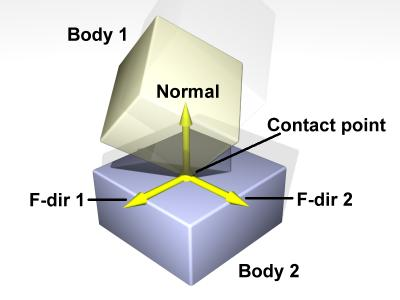
\includegraphics[scale = 0.7, width=\textwidth]{contact.jpg}
    \caption{Body interaction causing friction}
\end{figure}

Where $F_c$ is the Coulomb friction force, $v$ is the sliding speed, $\mu$ is the coefficient of friction, $N$ is the 
normal contact force and $F_{app}$ is the applied force on the body. \\

\section{URDF and SDF}
URDF (\textit{Unified Robot Description Format}) is an XML format for representing a robot model used by ROS. \\
A number of different packages and components compose URDF: \\

\begin{figure}[H]
    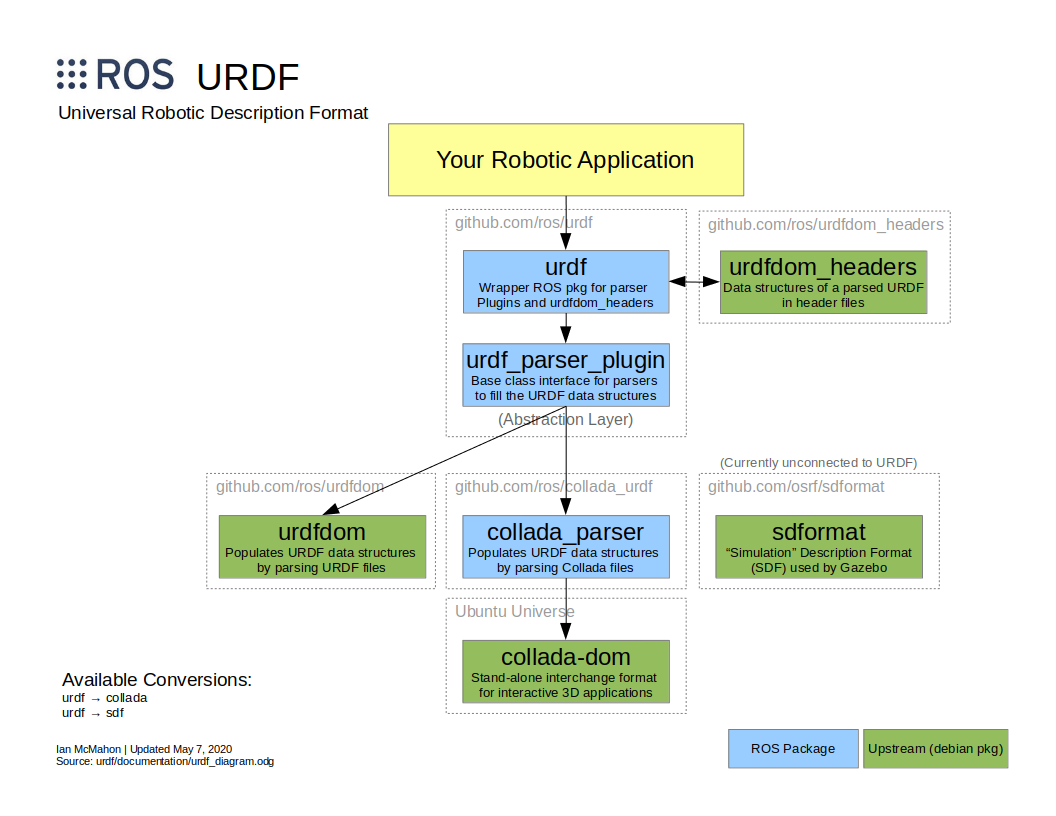
\includegraphics[width=\textwidth]{urdf_diagram.png}
    \caption{URDF description}
\end{figure}

URDF can only specify the kinematic and dynamic properties of a single robot in isolation, it cannot specify the pose 
of the robot itself with respect to the world it is placed in.\\
URDF is not a universal description format since it cannot specify joint loops (parallel linkages), and it lacks the possibility 
of specifying friction and other dynamic properties.\\
For the reasons above, Gazebo uses another XML format called SDF (\textit{Simulation Description Format}) which 
is a complete description for everything from the world level down to the robot level.\\ 
It has been developed also a macro language called XACRO (\textit{XML Macro}) to make it easier to maintain the robot description 
files, increase their readability, and to avoid duplication of code in the robot description files.
In our case, the model is described using XACRO files, and then it is converted to SDF by the \textit{gazebo\_ros} package.
Finally, it is spawned it in the Gazebo simulated world. \\
The basic building blocks for describing a robot using URDF/SDF are \textit{links} and \textit{joints}.

\subsection{Links}
In URDF/SDF, a \textit{Link}\footnote{Visit \url{https://wiki.ros.org/urdf/XML/link} for a detailed description} 
element describes a rigid body with an inertia, visual features, and collision properties. \\

\begin{figure}[H]
    \centering
    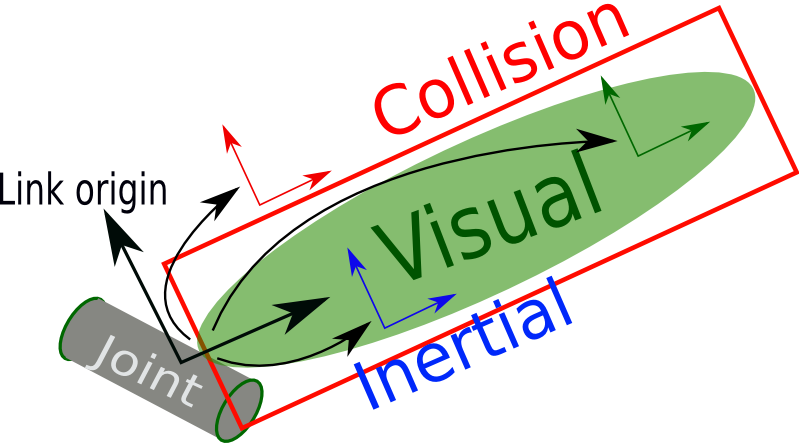
\includegraphics[scale=2]{inertial.png}
    \caption{Link schematic}
\end{figure}

Each \textit{link} element is composed by three main parts (encapsulated in their respective XML tags): 
\begin{itemize}
    \item \textit{Inertial} in which we specify the link mass, position of its center of mass, and its central inertia properties;
    \item \textit{Visual} in which we describe the shape of the object (e.g. box, cylinder) for visualization purposes. 
            We can also use multiple instances of <visual> tags for the same link to define the shape in a constructive way.
    \item \textit{Collision} in which we list the collision properties of a link, which are usually different from the visual ones. 
            In fact, simpler collision models are often used to reduce computation time. \\
            Also in this case, we can also use multiple instances of <collision> tags for the same link to define
            the desired shape in a constructive way.     
\end{itemize}


\subsection{Joints}
The \textit{joint}\footnote{Visit \url{https://wiki.ros.org/urdf/XML/joint} for a detailed description} 
element describes the kinematics, dynamics and safety limits of a joint connecting together two link objects.\\

\begin{figure}[H]
    \centering
    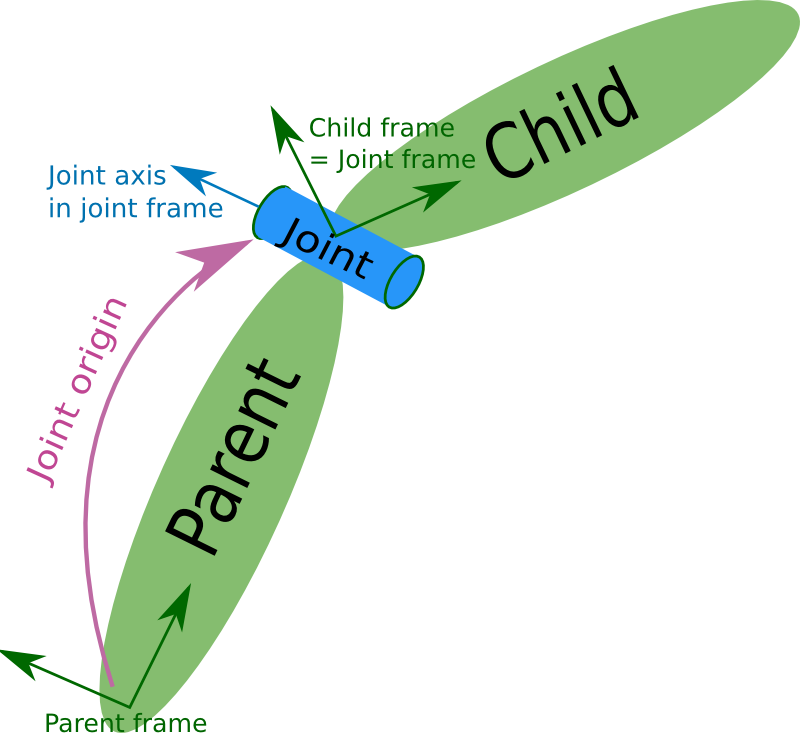
\includegraphics[scale=0.3]{joint.png}
    \caption{Joint schematic}
\end{figure}

Using the attribute \textit{type} we can specify the type of the joint as one of the following:
\begin{itemize}
    \item \textbf{revolute} — a hinge joint that rotates along the provided axis and has a limited range
                             specified by the upper and lower limits;
    \item \textbf{continuous} — a continuous hinge joint that rotates around the provided axis and has no upper and lower limits;
    \item \textbf{prismatic} — a sliding joint that slides along the axis, and has a limited range 
                                specified by the upper and lower limits;
    \item \textbf{fixed} — this is not really a joint because it cannot move since all degrees of freedom are locked. 
                            This type of joint is used to rigidly attach links together;
    \item \textbf{floating} — this joint allows motion for all 6 degrees of freedom;
    \item \textbf{planar} — this joint allows motion in a plane perpendicular to provided the axis. 
\end{itemize} 
Using <parent> and <child> XML elements, we can define which links (rigid bodies) are attached together through the joint. 

\subsection{URDF in Gazebo}
In order to use a robot described using URDF within Gazebo, it is mandatory that all links have an \textit{<inertial>} element. \\
Optionally, we can introduce additional information appending \textit{<gazebo>} elements to the links (e.g., to add sensor plugins
to convert colors to Gazebo format, ...), or to the joints (e.g., to set proper damping dynamics, add actuator control plugins, 
...).\footnote{Refer to \url{http://classic.gazebosim.org/tutorials?tut=ros_urdf} for a detailed guide on the conversion}


\section{RACECAR model description}
In this section we are going to explain the structure of the \textit{RACECAR project} developed by MIT, by focusing on 
the model the robot and on its simulation made by using Gazebo. \\
The robot is composed by nine links: a chassis, four wheels, two steering hinges, one Hokuyo LIDAR sensor and one camera;
and by eight joints: four for the wheels, two for the steering mechanism, and two for connecting the camera and the 
LIDAR to the car.\\

% racecar schematic
\begin{figure}[H]
    \makebox[\textwidth][c]{
    \begin{tikzpicture}[x=0.3cm,y=0.3cm] %set unit size along axes
        % axes (following Gazebo reference system)
        \draw[gray, opacity = 0.5,->] (0,-2) -- (0,5) node[right] {$x$};
		\draw[gray, opacity = 0.5,->] (2,0) -- (-5,0) node[above] {$y$};
		\draw[gray, opacity = 0.5] (0,0) node[below right] {o};

        %%% chassis %%%
        % rear left part
        \draw[very thick, BurntOrange] (-7,-4) -- (7,-4);
        \draw[very thick, BurntOrange] (-9,-2) -- (-9,-0.5);
        \draw[very thick, BurntOrange] (-9,-2) to[out=-90,in=180] (-7,-4); %rear left corner
        %rear left wheel axis
        \draw[very thick, BurntOrange] (-9,-0.5) -- (-10,-0.5);
        \draw[very thick, BurntOrange] (-10,-0.5) -- (-10,0.5);
        \draw[very thick, BurntOrange] (-10,0.5) -- (-9,0.5);
        %left part
        \draw[very thick, BurntOrange] (-9,0.5) -- (-9,23.5);
        \draw[very thick, BurntOrange] (-9,23.5) to[out=90,in=180] (-7,+25.5); %middle left corner
        \draw[very thick, BurntOrange] (-7,25.5) -- (-6,25.5);
        \draw[very thick, BurntOrange] (-6,25.5) -- (-6,32);
        %front left wheel axis
        \draw[very thick, BurntOrange] (-6,32) -- (-10,32);
        \draw[very thick, BurntOrange] (-10,32) -- (-10,33);
        \draw[very thick, BurntOrange] (-10,33) -- (-6,33);
        %front side
        \draw[very thick, BurntOrange] (-6,33) -- (-6,34.5);
        \draw[very thick, BurntOrange] (-6,34.5) to[out=90,in=180] (-4,36.5); %top left corner
        \draw[very thick, BurntOrange] (-4,36.5) -- (4,36.5);
        \draw[very thick, BurntOrange] (4,36.5) to[out=0,in=90] (6,34.5); %top right corner
        \draw[very thick, BurntOrange] (6,34.5) -- (6,33);
        %front right wheel axis
        \draw[very thick, BurntOrange] (6,32) -- (10,32);
        \draw[very thick, BurntOrange] (10,32) -- (10,33);
        \draw[very thick, BurntOrange] (10,33) -- (6,33);
        %right part
        \draw[very thick, BurntOrange] (9,0.5) -- (9,23.5);
        \draw[very thick, BurntOrange] (9,23.5) to[out=90,in=0] (7,+25.5); %middle left corner
        \draw[very thick, BurntOrange] (7,25.5) -- (6,25.5);
        \draw[very thick, BurntOrange] (6,25.5) -- (6,32);
        %rear right wheel axis
        \draw[very thick, BurntOrange] (9,-0.5) -- (10,-0.5);
        \draw[very thick, BurntOrange] (10,-0.5) -- (10,0.5);
        \draw[very thick, BurntOrange] (10,0.5) -- (9,0.5);
        % rear right part
        \draw[very thick, BurntOrange] (9,-2) -- (9,-0.5);
        \draw[very thick, BurntOrange] (9,-2) to[out=-90,in=0] (7,-4); %rear left corner

        %%% wheels %%%
        %rear left wheel%
        \draw[very thick, BlueGreen] (-10,-5) -- (-10,5);
        \draw[very thick, BlueGreen] (-10,-5) -- (-14.5,-5);
        \draw[very thick, BlueGreen] (-14.5,-5) -- (-14.5,5);
        \draw[very thick, BlueGreen] (-14.5,5) -- (-10,5);
        %top left wheel%
        \draw[very thick, BlueGreen] (-10,27.5) -- (-10,37.5);
        \draw[very thick, BlueGreen] (-10,27.5) -- (-14.5,27.5);
        \draw[very thick, BlueGreen] (-14.5,27.5) -- (-14.5,37.5);
        \draw[very thick, BlueGreen] (-14.5,37.5) -- (-10,37.5);
        %rear right wheel%
        \draw[very thick, BlueGreen] (10,-5) -- (10,5);
        \draw[very thick, BlueGreen] (10,-5) -- (14.5,-5);
        \draw[very thick, BlueGreen] (14.5,-5) -- (14.5,5);
        \draw[very thick, BlueGreen] (14.5,5) -- (10,5);
        %top right wheel%
        \draw[very thick, BlueGreen] (10,27.5) -- (10,37.5);
        \draw[very thick, BlueGreen] (10,27.5) -- (14.5,27.5);
        \draw[very thick, BlueGreen] (14.5,27.5) -- (14.5,37.5);
        \draw[very thick, BlueGreen] (14.5,37.5) -- (10,37.5);

        %steering hinges (circles of radius 1)
        \draw[very thick, Orchid] (-10, 32.5) circle[radius=1];
        \draw[very thick, Orchid] (10, 32.5) circle[radius=1];

        %%% legend %%%
	    \matrix [draw] at (current bounding box.east) {
        \node [circle, scale = 0.8, draw, fill= BurntOrange,label=right:\tiny Chassis] () {}; \\
        \node [circle, scale = 0.8, draw, fill= BlueGreen,label=right:\tiny Wheels] () {}; \\
        \node [circle, scale = 0.8, draw, fill= Orchid,label=right:\tiny Steering hinges] () {}; \\
        };
        
        \draw[thick, {Bar}-{Bar}] (16,-8) -- (17,-8) node[midway, above]{\small \SI{1}{\cm}};

        %%% measures %%%
        %back
        \draw[<->] (-9,-7) -- (9,-7) node[midway, above]{\small \SI{18}{\cm}};
        \draw[dashed, gray, opacity=0.5] (-9,-7) -- (-9,-2);
        \draw[dashed, gray, opacity=0.5] (9,-7) -- (9,-2);

        \draw[<->] (-10,-9) -- (10,-9) node[midway, above]{\small \SI{20}{\cm}};
        \draw[dashed, gray, opacity=0.5] (-10,-9) -- (-10,-5);
        \draw[dashed, gray, opacity=0.5] (10,-9) -- (10,-5);

        %wheel
        \draw[<->] (10,6) -- (14.5,6) node[midway, above]{\small \SI{4.5}{\cm}};
        \draw[dashed, gray, opacity=0.5] (10,6) -- (10,5);
        \draw[dashed, gray, opacity=0.5] (14.5,6) -- (14.5,5);

        \draw[<->] (15.5, -5) -- (15.5, 5) node[midway, right]{\small \SI{10}{\cm}};
        \draw[dashed, gray, opacity=0.5] (15.5, -5) -- (14.5,-5);
        \draw[dashed, gray, opacity=0.5] (15.5, 5) -- (14.5,5);

        %front
        \draw[<->] (-6,39) -- (6,39) node[midway, above]{\small \SI{12}{\cm}};
        \draw[dashed, gray, opacity=0.5] (-6, 39) -- (-6, 34.5);
        \draw[dashed, gray, opacity=0.5] (6, 39) -- (6, 34.5);

        \draw[<->] (-10,41) -- (10,41) node[midway, above]{\small \SI{20}{\cm}};
        \draw[dashed, gray, opacity=0.5] (-10, 41) -- (-10, 37.5);
        \draw[dashed, gray, opacity=0.5] (10, 41) -- (10, 37.5);

        %side
        \draw[<->] (-16, 0) -- (-16, 32.5) node[midway, right]{\small \SI{32.5}{\cm}};
        \draw[dashed, gray, opacity=0.5] (-16, 0) -- (-14.5, 0);
        \draw[dashed, gray, opacity=0.5] (-16, 32.5) -- (-14.5, 32.5);

        \draw[<->] (-18, -4) -- (-18, 25.5) node[midway, left]{\small \SI{29.5}{\cm}};
        \draw[dashed, gray, opacity=0.5] (-18, -4) -- (-7, -4);
        \draw[dashed, gray, opacity=0.5] (-18, 25.5) -- (-7, 25.5);
        \draw[<->] (-18, 25.5) -- (-18, 36.5) node[midway, left]{\small \SI{11}{\cm}};
        \draw[dashed, gray, opacity=0.5] (-18, 36.5) -- (-4, 36.5);


    \end{tikzpicture}}
    \caption{RACECAR links schematic}
    \label{fig:racecar}
\end{figure}

\subsection{RACECAR links}
\subsubsection{Chassis}
The robot chassis weights \SI{4}{\kilogram} and has an irregular shape (see schematic in \ref{fig:racecar}); 
it is placed \SI{5}{\cm} above the ground (\SI{0.05}{\metre} offset on the $z$ axis). Since there is 
no <collision> element, all collisions with the chassis are ignored.\\ 
The inertial matrix is: 
$$
\begin{bmatrix}
0.010609 & 0 & 0 \\
0 & 0.050409 & 0 \\
0 & 0 & 0.05865 \\
\end{bmatrix}
\quad
$$
It is a frictionless surface ($\mu_{1} = \mu_{2} = 0$), but has spring constant equals to \SI[per-mode = symbol]{1e7}{\newton\per\metre}
and a damping constant of \SI[per-mode = symbol]{1.0}{\kilogram\per\second}.

\subsubsection{Wheels}
Each one of the four wheels, weighting \SI{0.34}{\kilogram}, has a cylindrical shape with rounded borders defined 
by a custom STL (\textit{STereo Lithography interface format}) file. \\
The inertial matrix is reported here: 
$$
\begin{bmatrix}
0.00026046 & 0 & 0 \\
0 & 0.00026046 & 0 \\
0 & 0 & 0.00041226 \\
\end{bmatrix}
\quad
$$
Each wheel has also two friction coefficients, $\mu_{1}$ and $\mu_{2}$, both set to $1$; these coefficients 
are referring to the principal contact directions along the contact surface.
Furthermore, we have a spring constant of \SI[per-mode = symbol]{1e7}{\newton\per\metre} and a 
damping constant of \SI[per-mode = symbol]{1.0}{\kilogram\per\second}. \\
Since we are interested in the ground tire interaction, it is necessary to specify the first friction direction 
in the local reference frame along which frictional force is applied. Such vector must be of unit length and perpendicular 
to the contact normal, it is typically tangential to the contact surface: rear wheels have a friction direction 
vector equal to 
$\left[\begin{smallmatrix} 1 & 0 & 0 \end{smallmatrix}\right]$, instead front wheels have a friction 
direction vector equal to $\left[\begin{smallmatrix} 0 & 0 & 1 \end{smallmatrix}\right]$. \\
Each wheel has its own collision space, it is delimited by a cylinder \SI{4.5}{\cm} long and having a 
radius of \SI{5}{\cm}. The origin of the collision spaces for right wheels are shifted by
 $\left[\begin{smallmatrix} 0 & 0 & 0.0225 \end{smallmatrix}\right]$,
instead the origin of the collision spaces for the left wheels are shifted by
 $\left[\begin{smallmatrix} 0 & 0 & -0.0225 \end{smallmatrix}\right]$.
These translations, performed with respect to the joints frames (connecting the wheels to the chassis), are necessary
to align the generated collision cylinders with the visual geometries.
\footnote{At a first glance, different translations of the wheels along the $z$ axis may appear odd. However, it is motivated by the fact that 
the wheels joints have previously been rotated around the $x$ axis.}

\subsubsection{Steering Hinges}
The RACECAR model has two steering hinges for the front wheels, both have identical geometry: they are modeled as spheres. \\
The steering hinges only have visual properties specified, while no collision spaces are provided. \\
Each one weights \SI{0.1}{\kilogram}, and has the following inertial matrix:
$$
\begin{bmatrix}
4E-06 & 0 & 0 \\
0 & 4E-06 & 0 \\
0 & 0 & 4E-06 \\
\end{bmatrix}
\quad
$$

\subsubsection{Hokuyo Laser}
The RACECAR model is also equipped with a Hokuyo LIDAR sensor. To include it in the simulation, a laser Gazebo plugin is used\footnote{Visit 
\url{https://classic.gazebosim.org/tutorials?tut=ros_gzplugins\#Laser} for more information}. \\
The laser is set to have an update rate of \SI{40}{\hertz} with $1081$ simulated rays scanning the horizontal plane from angle \SI{-2.356}{\radian}
to \SI{2.356}{\radian}; the distance at which it can detect obstacles ranges from a minimum of \SI{10}{\cm} to a maximum of 
\SI{10}{\metre}, with a resolution of \SI{1}{\cm}.\\
To have a simulation as close to the real world as possible, a Gaussian noise is introduced in the readings of the LIDAR sensor: with a mean 
of \SI{0.0}{\metre} and a standard deviation of \SI{0.01}{\metre}, 99.7\% of readings are within \SI{0.03}{\metre} of the true distance. \\ 
The sensor weights \SI{0.13}{\kilogram} and its inertial matrix is :
$$
\begin{bmatrix}
4E-06 & 0 & 0 \\
0 & 4E-06 & 0 \\
0 & 0 & 4E-06 \\
\end{bmatrix}
\quad
$$
The collision space delimited by a cube having side long \SI{0.1}{\metre}.

\subsubsection{ZED Camera}
The last sensor attached to the RACECAR model is a ZED RGB camera, simulated with a camera Gazebo plugin\footnote{Visit 
\url{https://classic.gazebosim.org/tutorials?tut=ros_gzplugins\#Camera} for more information}.\\
This sensor has an update rate of \SI{30.0}{\hertz}, the resolution of the acquired image is $640$x$480$ in $B8G8R8$ color space.
Objects closer than the camera near clipping plane (placed at \SI{0.02}{\metre}) or further than the camera far clipping plane 
(positioned at \SI{300}{\metre}) won't be visible in the picture. \\
As in the case of the LIDAR, we have an artificial Gaussian noise with a mean 
of 0 and a standard deviation of 0.007 affecting the measurements. Such noise is sampled independently per pixel on each frame,
and it is added to each of its color channels (having values lying in the range [0,1]). \\
The sensor weights \SI{1e-5}{\kilogram}, and its inertial matrix is:
$$
\begin{bmatrix}
1E-6 & 0 & 0 \\
0 & 1E-06 & 0 \\
0 & 0 & 1E-06 \\
\end{bmatrix}
\quad
$$
The collision and visual spaces coincide, they are described by a box of dimensions 
\SI{0.033}{\metre} x \SI{0.175}{\metre} x \SI{0.030}{\metre}. \\

\subsection{RACECAR joints}
\subsubsection{Wheel joints}
All four wheel joints are continuous joints which allow the tires to rotate freely. \\
The effort limit on each joint is \SI[inter-unit-product =\ensuremath{\cdot}]{10}{\newton\metre}, while the 
velocity limit is \SI[per-mode = symbol]{100}{\radian \per \second}.
The joints are rotated by $\frac{\pi}{2}$ with respect to the $x$ axis so that the attached wheels end up in the 
correct alignment. In fact, the tires are described (in the STL file) as cylinders with their bases parallel to the ground,
so we need the \SI{90}{\degree} rotation to make them perpendicular to the terrain. \\
Apart from the positioning in space, the only difference between front wheels joints and rear wheel joints is their parent link:
the former are attached to the steering hinges, while the latter are directly connected to the chassis.

\subsubsection{Steering hinge joints}
Right and left steering hinges are connected to the chassis through two revolute joints. \\
Because of the joints nature, the range of motion is limited between a minimum and a maximum angle:
in this case, \SI{-1.0}{\radian} and \SI{1.0}{\radian}.
Originally, the effort limit was set to \SI[inter-unit-product =\ensuremath{\cdot}]{10}{\newton\metre} in order to simulate
a realistic steering dynamics. Since the feedback linearization law we used required to have an instantaneous steering 
mechanism, we increased such parameter to \SI[inter-unit-product =\ensuremath{\cdot}]{1000}{\newton\metre}, drastically 
reducing the steering time. \\
Finally, the velocity limit is \SI[per-mode = symbol]{100}{\radian \per \second}.

\subsubsection{Hokuyo laser Joint}
The laser sensor is attached to the chassis by a fixed joint, thus all its degrees of freedom are locked. This type 
of joint does not require to specify any additional information apart from the position and the connected elements.

\subsubsection{ZED camera joint}
In a similar way as the laser sensor, the camera is connected to the chassis through a fixed joint.
Because of that, only the position, the parent and child connections are specified.

\section{Plugins}
RACECAR model is enriched with functionalities that can control the several components specified before in the 
model description section.\\
These functionalities are implemented as plugins: chunks of code compiled as shared libraries 
and then inserted into the simulation. A plugin has direct access to Gazebo functionalities through C++ classes.\\
Plugins are used because of several advantages: they let developers control almost any aspect of Gazebo,
they are self-contained routines that are easily shared, and they can be inserted and removed quickly from a running system.\\
There are six different types of plugins and each of them is managed by different Gazebo components, these types are:
\begin{itemize}
    \item World, to control the simulated world;
    \item Model, to control a specific model;
    \item Sensor, to simulate a sensor behaviour;
    \item System, to introduce functionalities during Gazebo startup;
    \item Visual, to modify the visual representation of the simulation;
    \item GUI, to develop additional elements for the Gazebo interface.
\end{itemize}
A plugin type should be chosen based on the desired functionality to implement.\footnote{Visit 
\url{https://classic.gazebosim.org/tutorials?tut=ros_gzplugins} for additional information}\\
In this section we will analyze every plugin present in the /textit{RACECAR project} by specifying characteristics, 
functionalities and connections between components.

\subsection{gazebo\_ros\_control plugin}
The \textit{gazebo\_ros\_control}\footnote{See \url{https://classic.gazebosim.org/tutorials?tut=ros_control} for more information}
plugin is an adapter of the ros\_control library for Gazebo.\\
The \textit{ros\_control}\footnote{See \url{https://wiki.ros.org/ros_control} for more information} 
package takes as input the joint set data from the robot actuators and an input set point, then it
uses a PID control loop feedback mechanism to control the output. Such value, which is typically an effort,
is then sent to the robot actuators. \\
When there is not a one-to-one mapping of joint positions, efforts, etc... it is needed to use \textit{transmissions}:
interfaces that map effort/flow variables to output effort/flow variables while preserving power. \\
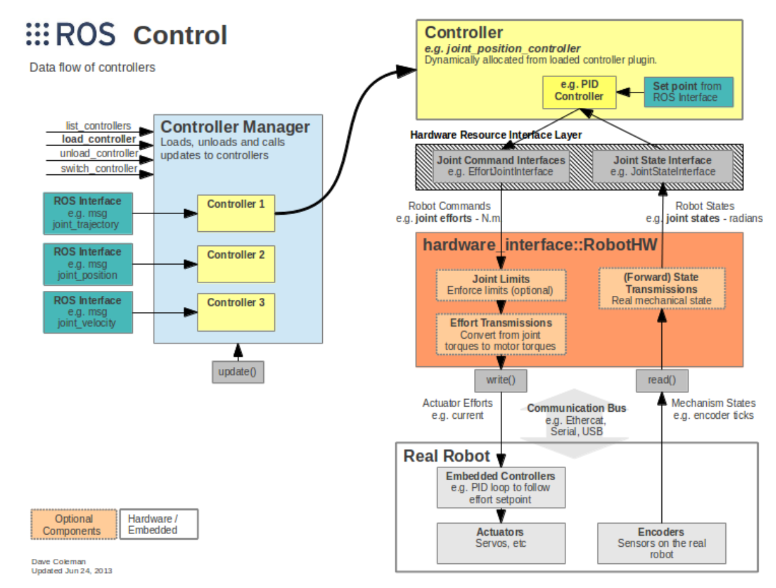
\includegraphics[width=\textwidth]{ros_control.png}\\
In the \textit{RACECAR project} we have six \textit{effort\_controllers}\footnote{Relative configuration can be found at 
\path{/catkin_ws/src/mit_racecar/racecar_gazebo/racecar_control/config/racecar_control.yaml}} form the ros\_control library,
they are PID controllers acting on the joint variables:
\begin{itemize}
    \item four, one for each wheel, of type \textit{joint\_velocity\_controller}, which receive a velocity setpoint
          and sends an effort output. They are pure proportional controllers with a gain of $1.0$ for the rear wheels, 
          and a gain of $0.5$ for the front tires;  
    \item two, one for each steering hinge, of type \textit{joint\_position\_controller}, which receive a position 
          input and sends an effort output. They are PD controllers with parameters $K_p = 1.0$ and $K_d = 0.5$;
\end{itemize}

The gazebo\_ros\_control plugin provides default ros\_control interfaces, and it also provides a pluginlib-based
interface to implement custom interactions between Gazebo and ros\_control for simulating more complex mechanisms.\\
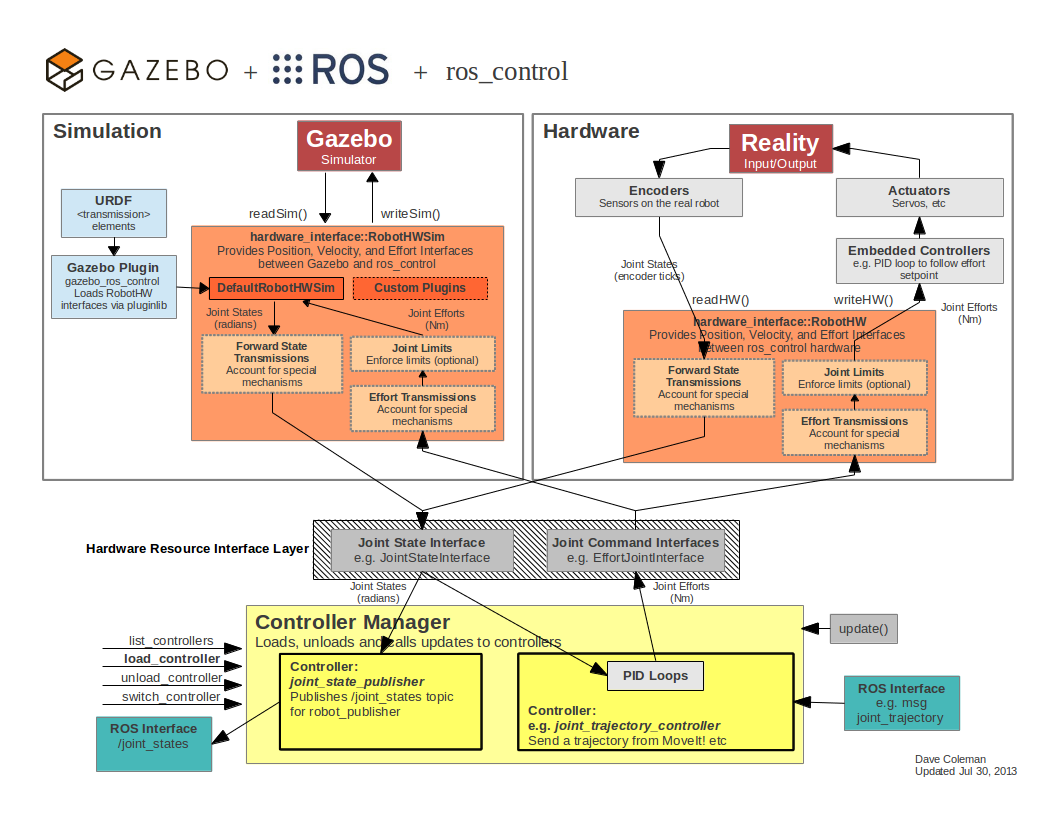
\includegraphics[width=\textwidth]{Gazebo_ros_transmission.png}\\
In order to use ros\_control within Gazebo, we need to enrich the URDF description adding <transmission> elements
in order to link actuators with joints. In our model, we have six transmissions: four to connect each wheel to a 
motor (with a mechanical reduction of $1$), and two connecting each steering hinge to a dedicated motor (also in
this case the mechanical reduction is $1$). \\
Finally, we add to the URDF file the gazebo\_ros\_control plugin by specifying the library filename ("libgazebo\_ros\_control.so")
and its parameters like a desired "robotNamespace".

\subsection{Laser plugin}
The Hokuyo laser plugin is specified in a \textit{Sensor} tag. It refers to the library 
\textit{libgazebo\_ros\_laser.so} which takes the role of controller of the laser 
(named \textit{gazebo\_ros\_hokuyo\_controller}).\\
This controller gathers range data from a simulated ray sensor, publishes range data using 
\textit{sensor\_msgs::LaserScan} messages on the ROS topic named \textit{/scan}.

\subsection{Camera plugin}
Similarly as the laser scan plugin the camera plugin is specified in a \textit{Sensor} tag. It refers
to the library \textit{libgazebo\_ros\_camera.so} which allows to control this sensor (the controller
is named \textit{camera\_controller}).\\
The camera publishes image messages on \textit{camera/zed/rgb/image\_rect\_color} ROS topic, while the
info messages are published on \textit{camera/zed/rgb/camera\_info}.\\
The coordinate frame where the image is published (tf tree) is \textit{camera\_link}.

\section{racecar\_gazebo code description}
In the previous sections we have illustrated how the model has been designed and its characteristics. In this
section we want to explain how the code is organized and the technical details of the implementation.\\
We will focus only on the \textit{racecar\_gazebo} package inside \textit{mit\_racecar}.

\subsection{racecar\_description}
The \textit{racecar\_description} package contains all specifications and files useful
to describe the car and the environments of the simulation.\\
In the \textit{urdf} folder there are four different XML files:
\begin{itemize}
    \item \textbf{macros.xacro}
    containing macros definitions for inertial parameters, geometries and transmissions
    for all the elements composing the car model. The usage of a xacro file allows to have a more readable 
    and organized code in the main URDF files.
    \item \textbf{materials.xacro} with the specification of the materials used in the car construction within
    Gazebo (in this case each material is simply determined by a RGB color that will be used for the visualization). 
    \item \textbf{racecar.xacro} which is the main description file. It contains all links, joints and transmissions
    composing the car model.\\
    It also includes all the other macro files and the Gazebo one.
    \item \textbf{racecar.gazebo} with friction parameters, plugin settings and all the additional 
    information needed to use URDF within a Gazebo simulation.
\end{itemize}
In the \textit{models} directory there are \textit{.config} and \textit{.sdf} files used to describe
the simulation environments. \\
The last folder is named \textit{meshes}, it contains \textit{.STL} and \textit{.dae} files which are the 3D models
of the car components used by Gazebo for the visual rendering.

\subsection{racecar\_gazebo}
In this package there are the files used to launch the Gazebo simulation.\\
In the \textit{worlds} folder we have several \textit{.worlds} files: they contain the description
of the available environments (worlds) in which the model can be simulated. \\
The second folder, named \textit{script}, contains the python implementation of \textit{gazebo\_odometry\_node}. 
This node is in charge of translating Gazebo status messages (coming from "/gazebo/link\_states" topic) to odometry data,
and then publishing it on "/vesc/odom" ROS topic at a \SI{20.0}{\hertz} rate. \\
The last folder is named \textit{launch} and contains one launch file for each world already implemented. \\
A launch file contains the list of ROS nodes to be spawned and their configuration; moreover, it can include
other \textit{.launch} files. Hence, we have a quick and tidy way to start the entire simulation. \\
In the package there are five \textit{.launch} files; the main one is \textit{racecar.launch}, while the others
only differ for the world in which the simulation will take place. \\
File \textit{racecar.launch} contains the following parts:  
\begin{itemize}
    \item world selection: it is specified the \textit{.world} file which describes the simulation environment (in this case
          an empty flat plane);
    \item robot description generation: the \textit{.xacro} file containing the description of the car model is converted 
          to URDF format and loaded into the parameter server;
    \item racecar spawning: \textit{racecar\_spawn} node, from \textit{gazebo\_ros} package, reads the model URDF from 
          the parameter server and implements it in the simulation; 
    \item call to \textit{racecar\_control.launch}: which loads all the joints effort controllers and starts the 
          \textit{servo\_commands} node; 
    \item call to \textit{mux.launch}: which creates a multiplexer to the handle different commands, having different priorities,
          received by the car. 
    \item topic remapping: \textit{better\_odom} node, from \textit{topic\_tools} package, uses the "relay" functionality 
          to subscribe to \textit{/vesc/odom} and republish to \textit{/pf/pose/odom}. 
\end{itemize}

\subsection{racecar\_control}
This package contains the logic of the car controllers.\\
In the \textit{scripts} we have the implementation of two ROS nodes:
\begin{itemize}
    \item \textit{keyboard\_teleop}\\
    Which allows the user to manually control the car by sending commands using the keyboard: \textit{W} to go forward,
    \textit{S} to move in reverse, \textit{A} and \textit{D} for turning left and right respectively. 
    Pressing a different key will stop the car, and by using the combination \textit{CTRL-C} the node is terminated and
    the controller stopped.\\
    A message of type \textit{AckermannDriveStamped} containing speed, acceleration, jerk, steering\_angle 
    and steering\_angle\_velocity is then published on the \textit{/vesc/ackermann\_cmd\_mux/input/teleop} topic to
    be sent to the car command mutiplexer.
    \item \textit{servo\_commands}\\
    The main purpose of this node is to read the information published on the \textit{/racecar/ackermann\_cmd\_mux/output} 
    topic by the multiplexer, and forward it to the various link controllers. \\
    It publishes the desired speed, pre-multiplied by 10, to the four wheel velocity controller topics; while,
    to the two hinge position controllers, it is forwarded the steering angle setpoints.
\end{itemize}
The second folder is named \textit{config}, it contains only one file which is \textit{racecar\_control.yaml}.
 A YAML file loads node configuration parameters in the ROS parameter server, it contains the information 
 about type, joint name and PID (proportional-integral-derivative) gain of each controller to be implemented 
 using the ros\_control library.

The \textit{launch} directory contains three launch files regarding controller functionalities:
\begin{itemize}
    \item \textit{gazebo\_sim\_joy.launch}\\
    starts the simulation in the tunnel environment and calls \textit{teleop.launch} (see below);
    \item \textit{racecar\_control.launch}\\
    loads the joint controller configurations from \textit{racecar\_control.yaml} to parameter server:
    Then it instantiates a \textit{controller\_manager}: a node (implemented in ros\_control) capable of spawning, loading, 
    unloading and updating all the controllers specified in the configuration file (.yaml file).
    Finally, it starts the aforementioned servo\_commands node. \\
    In addition, this file includes also some remapping of the topics used by the robot state publisher 
    (robot\_state\_publisher node), the robot movements controller (servo\_commands node) and the odometry publisher;
    \item \textit{teleop.launch} \\
    starts the \textit{keyboard\_teleop} node to allow the user to manually control the model.
\end{itemize}

\newpage
\chapter{(Our) System Description}

\section{Scheme of the whole system}

\begin{tikzpicture}
\node[
	draw,
	fill=BlueGreen,
	minimum width=2cm,
	minimum height=1.5cm
] (tracker) {Trajectory Tracker};

\node[
	draw,
	fill=BlueGreen,
	minimum width=2cm,
	minimum height=1.5cm,
	right=4cm of tracker
] (refVelocity) {Compute Ref. Velocity};

\node[
	draw,
	fill=Green,
	minimum width=2cm,
	minimum height=1.5cm,
	below=3cm of tracker
] (model) {Model MIT/ODE};

\node[
	draw,
	fill=Yellow,
	minimum width=2cm,
	minimum height=1.5cm,
	below=3cm of refVelocity
] (controller) {Linearizer};

\draw[-{Triangle[scale=2]}]  (-3, +1/3) --  ($(tracker.west) + (0, +1/3)$)
	node[midway, above]{$x_{ref}$};
	
\draw[-{Triangle[scale=2]}]  (-3, -1/3) --  ($(tracker.west) + (0, -1/3)$)
	node[midway, above]{$y_{ref}$};

% ---

\draw[-{Triangle[scale=2]}] ($(tracker.east) + (0, +1/3)$) -- ($(refVelocity.west) + (0, +1/3)$)
	node[midway, above]{$x_{current}$};
	
\draw[-{Triangle[scale=2]}] ($(tracker.east) + (0, -1/3)$) -- ($(refVelocity.west) + (0, -1/3)$)
	node[midway, above]{$y_{current}$};
	
% ---
	
\draw[-{Triangle[scale=2]}] ($(refVelocity.south) + (-1/2, 0)$) -- ($(controller.north) + (-1/2, 0)$)
	node[midway, left]{$V_{Xp}$};
	
\draw[-{Triangle[scale=2]}] ($(refVelocity.south) + (+1/2, 0)$) -- ($(controller.north) + (+1/2, 0)$)
	node[midway, left]{$V_{Yp}$};

% ---

\draw[-{Triangle[scale=2]}] ($(controller.west) + (0, +1/2)$) -- ($(model.east) + (0, +1/2)$)
	node[midway, above]{$\phi$};
	
\draw[-{Triangle[scale=2]}] ($(controller.west) + (0, 0)$) -- ($(model.east) + (0, 0)$)
	node[midway, above]{$V$};
	
\draw[-{Triangle[scale=2]}] ($(controller.west) + (0, -1/2)$) -- ($(model.east) + (0, -1/2)$)
	node[midway, above]{$\omega$};

% ---

\draw[-{Triangle[scale=2]}] ($(model.north) + (-1/2, 0)$) -- ($(tracker.south) + (-1/2, 0)$)
	node[near end, left]{$x_{in}$}
	node[near start, left]{$x_{out}$};
	
\draw[-{Triangle[scale=2]}] ($(model.north) + (+1/2, 0)$) -- ($(tracker.south) + (+1/2, 0)$)
	node[near end, left]{$y_{in}$}
	node[near start, left]{$y_{out}$};
	
\draw[-{Triangle[scale=2]}] (model.south) |- ++ (0, -1) -| (controller.south)
	node[near start, above]{$\theta_{out}$};

\end{tikzpicture}

\vspace{1cm}

\begin{center}
	\begin{tabularx}{\textwidth}{|l|X|}
		\hline
		\textbf{Symbol} & \textbf{Meaning} \\
		\hline
		$x_{ref}, y_{ref}$ & Ref. position of the trajectory \\
		\hline
		$V_{Xp}, V_{Yp}$ & Required velocities of the point. They will be imposed by controller\\
		\hline
		$\phi$ & Steer degree of rotation \\
		\hline
		$V$ & Vector velocity \\
		\hline
		$\omega$ & Steer speed of rotation \\
		\hline
		$\theta_{out}$ & Car pose: rotation around center axis\\
		\hline
		$x_{out}, y_{out}$ & Car pose: x, y \\
		\hline
	\end{tabularx}
\end{center}

\vspace{1cm}

Note that "trajectory tracker" generated trajectories are hard-coded, even if $x_{ref}$ and $y_{ref}$ are shown as input parameters. The user can select the trajectory using YAML configuration file (which will be explained in the relative section).

\section{Topics}

\subsection{Scheme of topic publications/subscriptions}

\subsubsection{ROS Friction Model}

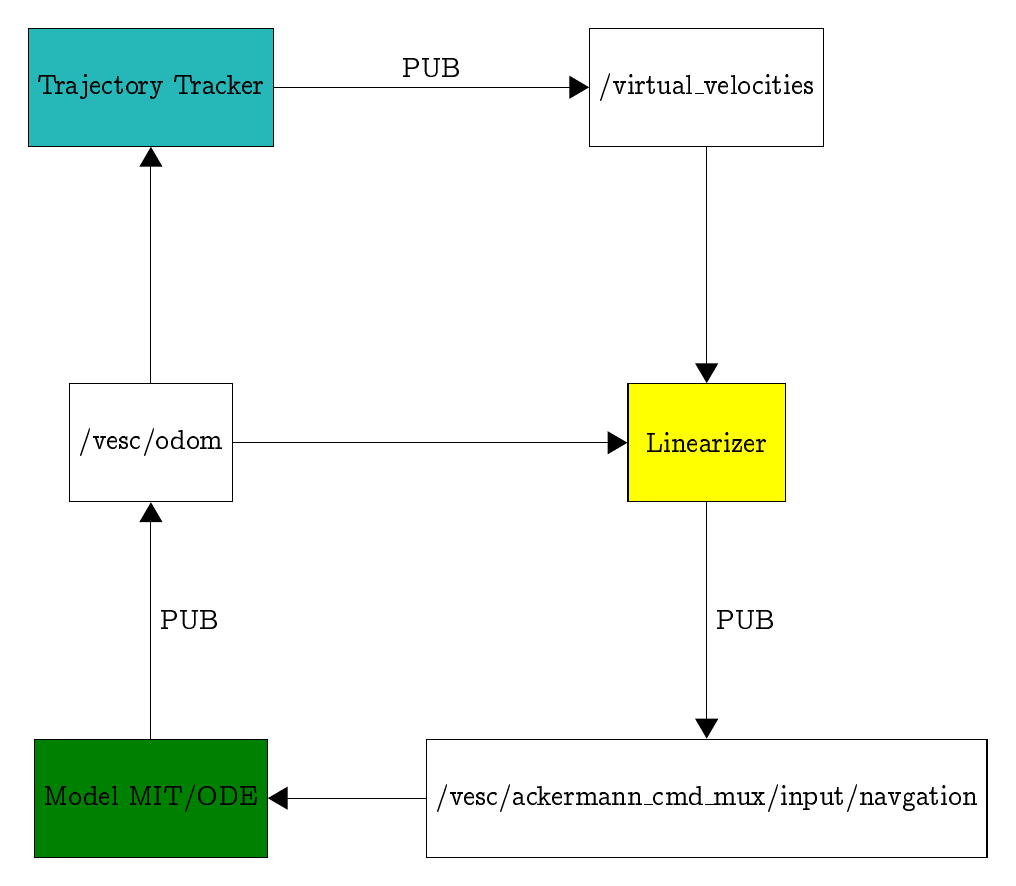
\begin{tikzpicture}
	
\node[
	draw,
	fill=BlueGreen,
	minimum width=2cm,
	minimum height=1.5cm
] (tracker) {Trajectory Tracker};

\node[
	draw,
	fill=White,
	minimum width=2cm,
	minimum height=1.5cm,
	right=4cm of tracker
] (virtualVel) {/virtual\_velocities};

\node[
	draw,
	fill=White,
	minimum width=2cm,
	minimum height=1.5cm,
	below=3cm of tracker
] (odom) {/vesc/odom};

\node[
	draw,
	fill=Yellow,
	minimum width=2cm,
	minimum height=1.5cm,
	below=3cm of virtualVel
] (controller) {Linearizer};

\node[
	draw,
	fill=Green,
	minimum width=2cm,
	minimum height=1.5cm,
	below=3cm of odom
] (model) {Model MIT/ODE};

\node[
	draw,
	fill=White,
	minimum width=2cm,
	minimum height=1.5cm,
	below=3cm of controller
] (ackermanCmd) {/vesc/ackermann\_cmd\_mux/input/navgation};

% ---

\draw[-{Triangle[scale=2]}] (tracker.east) -- (virtualVel.west)
	node[midway, above]{PUB};
	
\draw[-{Triangle[scale=2]}] (virtualVel.south) -- (controller.north)
	node[midway, right]{};
	
\draw[-{Triangle[scale=2]}] (controller.south) -- (ackermanCmd.north)
	node[midway, right]{PUB};
	
\draw[-{Triangle[scale=2]}] (ackermanCmd.west) -- (model.east)
	node[midway, above]{};
	
\draw[-{Triangle[scale=2]}] (model.north) -- (odom.south)
	node[midway, right]{PUB};
	
\draw[-{Triangle[scale=2]}] (odom.north) -- (tracker.south)
	node[midway, right]{};
	
\draw[-{Triangle[scale=2]}] (odom.east) -- (controller.west)
	node[midway, above]{};

\end{tikzpicture}


\subsection{Topics meaning}

\subsubsection{Common Topics}

\begin{center}
	\begin{tabularx}{\textwidth}{
			| >{\raggedright\arraybackslash}X
			| >{\raggedright\arraybackslash}X |
		}
		\hline
		/virtual\_velocities & Used by "trajectory tracker" to publish desired velocity components. These are read by controller in order to perform linearization and compute instructions for the model. \\
		\hline
		\makecell[lt]{/vesc/ackermann\_cmd\_mux \\ /input/navgation} & Contains AckermannDriveStamped messages sent by controller. These messages contains information for the racecar, about velocity and steering. \\
		\hline
		/vesc/odom & The model uses this topic to publish odometry information of the racecar (position and orientation). These data are used both by tracker and controller. The first one compute differences between actual car position and desired position imposed by trajectory. The last one reads z-axis orientation useful to perform linearization. \\
		\hline
	\end{tabularx}
\end{center}

There is another topic in which "trajectory tracker" publish, the \textit{/reference\_trajectory}. This is used to read trajectory information to perform debug and register data for analysis.

\vspace{1cm}

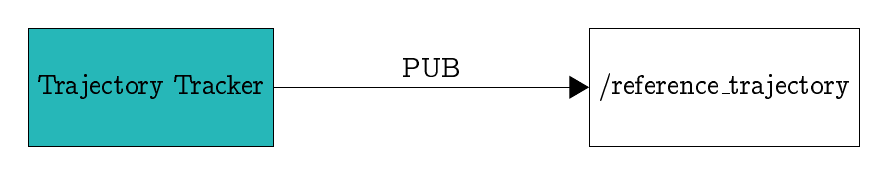
\begin{tikzpicture}
	
\node[
	draw,
	fill=BlueGreen,
	minimum width=2cm,
	minimum height=1.5cm
] (tracker) {Trajectory Tracker};

\node[
	draw,
	fill=White,
	minimum width=2cm,
	minimum height=1.5cm,
	right=4cm of tracker
] (reference) {/reference\_trajectory};

\draw[-{Triangle[scale=2]}] (tracker.east) -- (reference.west)
	node[midway, above]{PUB};

\end{tikzpicture}

%\subsubsection{Specific Topics}
%
%\begin{center}
%	\begin{tabularx}{\textwidth}{
%			| >{\raggedright\arraybackslash}X
%			| >{\raggedright\arraybackslash}X |
%		}
%		\hline
%		\makecell[lt]{/vesc/low\_level/ \\ ackermann\_cmd\_mux/output} & xyz \\
%		\hline
%	\end{tabularx}
%\end{center}

\chapter{Detailed Package Description}

\section{Package car\_dynamic\_linearizer}
\subsection{Intro}

Even if this package is not used, it's correct to do a description of the objective it should have reached.

The aim was to implement a dynamic controller, which perform exact linearization of the nonlinear bicycle dynamic model. To do this it needs more parameter respect to the kinematic one.

In addition, we put a scheme (\ref{fig:dynamic_model}) of the principal parameters and variables  used for linearization.

\begin{figure}[h]
	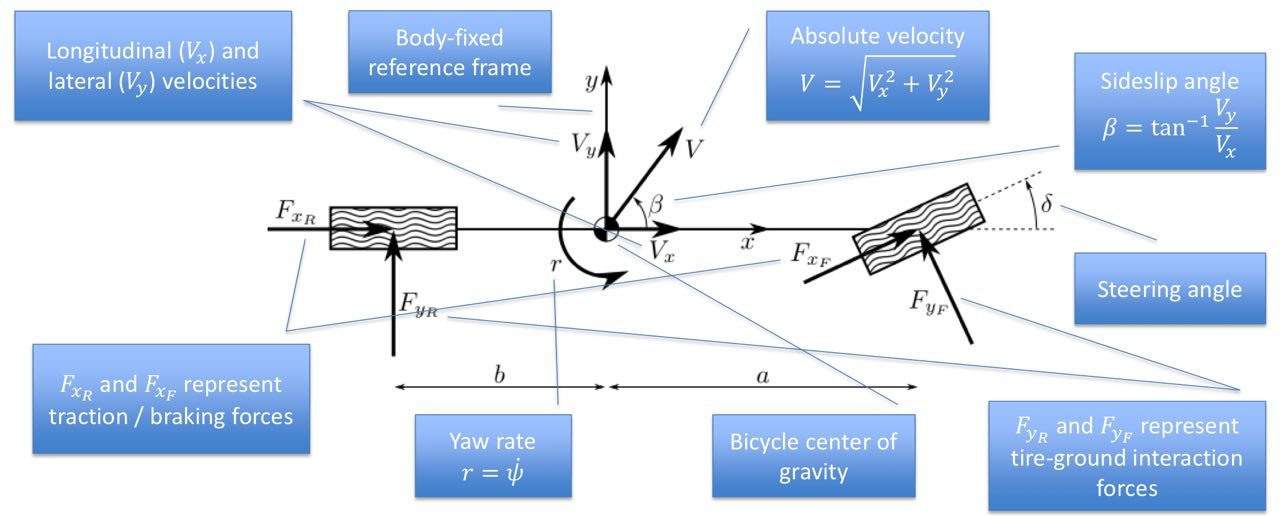
\includegraphics[scale=0.3]{dynamic_model}
	\caption{dynamic model with main parameters and variables}
	\label{fig:dynamic_model}
\end{figure}

\subsection{Configuration}

\begin{center}
	\begin{tabularx}{\textwidth}{
			| >{\raggedright\arraybackslash}X
			| >{\arraybackslash}X |
		}
		\hline
		\multicolumn{2}{|c|}{\textbf{Input values}} \\
		\hline
		$Vp_x$ & Point velocity x \\
		\hline
		$Vp_y$ & Point velocity y \\
		\hline
		$\psi$ & Yaw\footnote{In the System Scheme, this is represented by $\theta_{out}$} \\
		\hline
		$\dot{\psi}$ & Yaw rate\footnote{In the System Scheme, this is \textbf{not} represented (as we have used, for tests, only the kinematic model)} \\
		\hline
	\end{tabularx}
	
	\vspace{0.5cm}
	
	\begin{tabularx}{\textwidth}{
			| >{\raggedright\arraybackslash}X
			| >{\arraybackslash}X |
		}
		\hline
		\multicolumn{2}{|c|}{\textbf{Model parameters}} \\
		\hline
		$C_f$, $C_r$ & Viscuous friction coefficients \\
		\hline
		a, b & Distance between wheels center and Center of Gravity \\		
		\hline
		$M$ & Vehicle mass \\
		\hline
		$\epsilon$ & Distance between Center of Gravity and a point $P$, along the velocity vector. Linearization is done around point P. This parameter should be chosen empirically \\
		\hline
	\end{tabularx}
	
	\vspace{0.5cm}
	
	\begin{tabularx}{\textwidth}{
			| >{\raggedright\arraybackslash}X
			| >{\arraybackslash}X |
		}
		\hline
		\multicolumn{2}{|c|}{\textbf{Intermediate computed values}} \\
		\hline
		$\beta$ & Sideslip angle: $\tan^{-1}\left(\frac{Vp_y}{Vp_x}\right)$ \\
		\hline
	\end{tabularx}
	
	\vspace{0.5cm}
	
	\begin{tabularx}{\textwidth}{
			| >{\raggedright\arraybackslash}X
			| >{\arraybackslash}X |
		}
		\hline
		\multicolumn{2}{|c|}{\textbf{Output values}} \\
		\hline
		$V$ & Point absolute velocity \\
		\hline
		$\delta$ & Steering angle \\
		\hline
		$\omega$ & Steering speed \\
		\hline
	\end{tabularx}
\end{center}

\subsection{Launch}

There is a lunch file which \textbf{should be used to execute the node}. This contains also information about debugging level and loads configuration file.

\subsection{Node car\_dyn\_linearizer}

\[
\beta = \tan^{-1}\left(\frac{Vp_y}{Vp_x}\right)
\]
\[
\delta = \frac{MV}{C_f}\omega + \frac{C_f + C_r}{C_f}\beta - \frac{bC_r - aC_f}{C_f}\frac{\dot{\psi}}{V}
\]
\[
\begin{bmatrix}
	V \\
	\omega
\end{bmatrix}
=
\begin{bmatrix}
	\cos(\beta + \psi) & \sin(\beta + \omega) \\
	-\frac{\sin(\beta + \psi)}{\epsilon} & \frac{\cos(\beta + \psi)}{\epsilon} \\
\end{bmatrix}
\begin{bmatrix}
	Vp_x \\
	Vp_y
\end{bmatrix}
\]

\newpage

\section{Package car\_kinematic\_linearizer}
\subsection{Intro}

Before starting the explanation, we add a brief high level description of Quaternions, which are used in messages to represent orientations. Even a distinction between pose and position is done.

\textbf{Quaternion}: a different way to describe the orientation of a frame only. It's an alternative to Yaw, Pitch and Roll. A quaternion has four parameters: x, y, z, w. Pay attention, they are NOT a position vector.

\textbf{Position}: position of the robot in a 3D space.

\textbf{Pose}: position (3 DOF) + orientation (3 DOF).

In conclusion the pose has 6 D.O.F. which are: x, y, z, roll, pitch, yaw. Euler angles can be converted to quaternions, which are better. Transformation functions of ROS can do this conversion and the reverse one.

In addition, we put a scheme (\ref{fig:bicycle_vehicle}) of the principal parameters and variables  used for linearization.

\begin{figure}[h]
	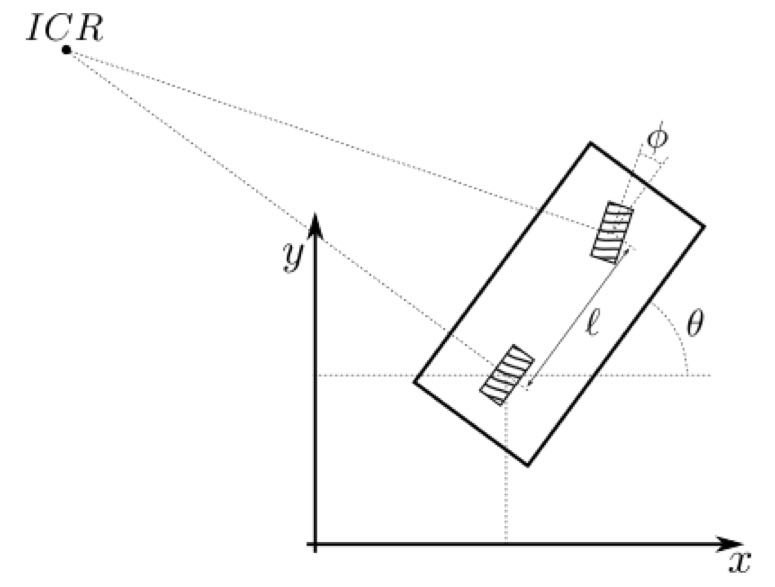
\includegraphics[scale=0.4]{kinematic_model}
	\caption{bicycle vehicle with main parameters and variables}
	\label{fig:bicycle_vehicle}
\end{figure}

\subsection{Configuration}

In the package there is a configuration file, containing: the parameter L, which represents distance between rear and front wheels; the parameter $\epsilon$, the distance between Center of Gravity and a point $P$, along the velocity vector. Linearization is done around point P. This parameter should be chosen empirically.

Both are used in the linearization.

\subsection{Launch}

There is a lunch file which \textbf{should be used to execute the node}. This contains also information about debugging level and loads configuration file.

\subsection{Node car\_kin\_linearizer}

\textbf{Node requirements}: distance between rear and front wheels as parameter.

The node has two callbacks:

\begin{itemize}
	\item One used to retrieve desired velocities of the point. These velocities are computed by trajectory tracker and published in \verb|/virtual_velocities| topic, subscribed by the controller node.
	\item One used to retrieve the orientation of the car around z axis. This is done reading from \verb|/vesc/odom|. The information retrieved are in the form of a quaternion and are converted into roll, pitch and yaw. Yaw is taken. In addition, even the speed around z axis is read (\verb|twist.angular.z|).
\end{itemize}

The node perform an exact linearization of the nonlinear bicycle cinematic model. The change of coordinates is applied as follows:

\[
V = V_{Xp}cos(\theta) + V_{Yp}sin(\theta)
\]

\[
\phi = \arctan\left(\frac{l}{\epsilon} \frac{ V_{Yp}cos(\theta) - V_{Xp}sin(\theta) }{ V_{Xp}cos(\theta) + V_{Yp}sin(\theta) }\right)
\]

Where 

\begin{itemize}
	\item $l$ is the distance between rear and front wheels
	\item $\epsilon$ is the distance between Center of Gravity and a point $P$
	\item $V_{Xp}$ and $V_{Yp}$ are the desired point velocities
	\item $\theta$ is the car orientation around z-axis
	\item $\phi$ is the steering angle
	\item $V$ is the driving velocity of the front wheel
\end{itemize}

In addition, the program compute the steering speed as $\omega = \frac{V}{l}\tan(\phi)$. This value is not used in the construction of the message because it's ignored by the model.

Once the linearization is performed an \verb|AckermannDriveStamped| message is built, containing $V$ and $\phi$. This message is published on \\ \verb|/vesc/ackermann_cmd_mux/input/navigation| topic, which is read by the model to make the car move. Linearization and command sending operations are repeated in a loop, which is the core of the node.

\newpage

\section{Package trajectoy\_tracker}
\subsection{Package description}

The \textit{trajectory\_tracker} package is responsible for two main tasks:
\begin{itemize}
	\item generating the setpoints of the desired trajectory;
	\item applying the control law to make the robot track such trajectory.
\end{itemize} 

\begin{figure}[H]
\makebox[\textwidth][c]{
\begin{tikzpicture}%[scale=0.6, every node/.style={scale=0.6}]
	\node[
		draw,
		fill=BlueGreen,
		minimum height=1.5cm
	] (generator) {\begin{tabular}{c} Trajectory \\ Generator \end{tabular}};
	
	\node[
		draw,
		fill=BlueGreen,
		minimum height=1.5cm,
		right= of generator,
	] (refTransform) {\begin{tabular}{c} Reference \\ Transformation \end{tabular}};
	
	\node[
		draw,
		fill=BlueGreen,
		minimum height=5cm,
		right = of refTransform,
		shift = {(0cm,-1.75cm)}
	] (trackingLaw) {\begin{tabular}{c} Trajectory \\ Tracker \end{tabular}};
	
	\node[
		draw,
		fill=BlueGreen,
		minimum height=1.5cm,
		below = 2 of refTransform
	] (outputTransform) {\begin{tabular}{c} Output \\ Transformation \end{tabular}};

	\node[
		draw,
		fill=Apricot,
		minimum height=1.5cm,
		below = 2 of generator
	] (odom) {\begin{tabular}{c} $/vesc/odom$ \end{tabular}};

	\node[
		draw,
		fill=Lavender,
		minimum height=1.5cm,
		right = of trackingLaw
	] (controlPackage) {\begin{tabular}{c} $car\_kinematic\_linearizer$ \end{tabular}};

	% trajectory generator node incoming arrows
	\draw[-{Triangle}]  ($(generator.north) + (-0.5, 1)$) -- ($(generator.north) + (-0.5, 0)$)
		node[above, pos=0.2]{\scriptsize \begin{tabular}{c} Desired \\ Trajectory \\ Shape \end{tabular}};

		\draw[-{Triangle}]  ($(generator.north) + (0.5, 1)$) -- ($(generator.north) + (0.5, 0)$)
		node[above, pos=0.10]{$t$};
	
	% reference transformation node incoming arrows
	\draw[-{Triangle}] ($(odom.east) + (0, +1/2)$) -- ++(0.55cm,0) |- ($(refTransform.south) - (0,1)$)  -- ($(refTransform.south)$);

	\draw[-{Triangle}] ($(generator.east) + (0, +1/3)$) -- ($(refTransform.west) + (0, +1/3)$)
		node[midway, above]{$x_{ref}$};
		
	\draw[-{Triangle}] ($(generator.east) + (0, -1/3)$) -- ($(refTransform.west) + (0, -1/3)$)
		node[midway, above]{$y_{ref}$};

	% trajectory tracking law node incoming arrows
	\draw[-{Triangle}] ($(refTransform.east) + (0, +1/3)$) -- ($(trackingLaw.west) + (0,1.75+1/3)$)
		node[midway, above]{$x_{P_{ref}}$};
		
	\draw[-{Triangle}] ($(refTransform.east) + (0, -1/3)$) -- ($(trackingLaw.west) + (0,1.75-1/3)$)
		node[midway, above]{$y_{P_{ref}}$};

	\draw[-{Triangle}] ($(outputTransform.east) + (0, +1/3)$) -- ($(trackingLaw.west) + (0,-1.75+1/3)$)
		node[midway, above]{$x_{P}$};
		
	\draw[-{Triangle}] ($(outputTransform.east) + (0, -1/3)$) -- ($(trackingLaw.west) + (0,-1.75-1/3)$)
		node[midway, above]{$y_{P}$};

	% output transformation node incoming arrows
	
	\draw[-{Triangle}] ($(odom.east) + (0, +1/2)$) -- ($(outputTransform.west) + (0,+1/2)$)
		node[midway, above]{$\theta$};
		
	\draw[-{Triangle}] ($(odom.east)$) -- ($(outputTransform.west)$)
		node[midway, above]{$x$};

	\draw[-{Triangle}] ($(odom.east) + (0, -1/2)$) -- ($(outputTransform.west) + (0,-1/2)$)
		node[midway, above]{$y$};

	% controlPackage node incoming arrows
	\draw[-{Triangle}] ($(trackingLaw.east) + (0, +1/3)$) -- ($(controlPackage.west) + (0,+1/3)$)
		node[midway, above]{$v_{x_{_{P}}}$};
		
	\draw[-{Triangle}] ($(trackingLaw.east) + (0, -1/3)$) -- ($(controlPackage.west) + (0,-1/3)$)
		node[midway, above]{$v_{y_{_{P}}}$};

	% legend
	\matrix [draw,below left] at (current bounding box.north east) {
 	\node [draw, fill= BlueGreen,label=right:\tiny trajectory\_tracker node] () {}; \\
	\node [draw, fill= Apricot,label=right:\tiny ROS topic] () {}; \\
	\node [draw, fill= Lavender,label=right:\tiny other package] () {}; \\
	};

\end{tikzpicture}}
\caption{trajectory\_tracker package schematic}
\end{figure}

The main components of the package are:
\begin{itemize}
	\item[\textcolor{BlueGreen}{$\blacksquare$}] \textbf{Trajectory Generator} which is in charge of computing the appropriate 
		setpoint given the desired trajectory shape and the time $t$ elapsed since the starting of the motion. \\
		The implemented trajectory shapes are:
		\begin{itemize}
			\item[$\blacktriangleright$] Line, a simple linear path described by equations:
				\[ x_{ref} = at \qquad (\dot{x_{ref}} = a) \]
				\[ y_{ref} = bt \qquad (\dot{y_{ref}} = b) \] 
				Where $a$ and $b$ determine the direction (the line is parallel to the direction vector $\vec{d}=(a,b)$) and the speed of the trajectory;
				
				\begin{figure}[H]
				\makebox[\textwidth][c]{
					\begin{tikzpicture}
						\draw[gray,very thin, opacity = 0.5] (-0.9,-0.9) grid (4.9,4.9) [step=0.25cm];
						\draw[->] (-1,0) -- (5,0) node[right] {$x$};
						\draw[->] (0,-1) -- (0,5) node[above] {$y$};
						\draw[] (0,0) node[below left] {O};

						\draw[-, color=Red, thick] (0,0) -- (3,5) node[above] {};
						\draw[->, thick] (2,1) -- (2.5145,1.857) node[above] {$\scriptstyle \vec{d}=(a,b)$};
					\end{tikzpicture}}
				\caption{Linear trajectory (where $\vec{d}=(3,5)$)}
				\end{figure}	

			\item[$\blacktriangleright$] Parabola, a parabolic path described by equations: 
				\[x_{ref} = 2at \qquad (\dot{x_{ref}} = 2a)\]
				\[y_{ref} = at^2 \qquad (\dot{y_{ref}} = 2at)\]
				Where $a$ is the focal length of the parabola;
				
				\begin{figure}[H]
				\makebox[\textwidth][c]{
					\begin{tikzpicture}
						\draw[gray,very thin, opacity = 0.5] (-0.9,-0.9) grid (6.9,4.9) [step=0.25cm];
						\draw[->] (-1,0) -- (7,0) node[right] {$x$};
						\draw[->] (0,-1) -- (0,5) node[above] {$y$};
						\draw[] (0,0) node[below left] {O};

						% draw parabola having a = 2
						\draw[thick, color = red ,variable=\t,domain=0.0:1.58, smooth]
							plot ({\t*2*2},{2*\t^2});
						\draw[-, thick] (0,0) -- (0,2) node[above right] {$F=(0,a)$};
						\fill (0,2)    circle (2pt);
					\end{tikzpicture}}
				\caption{Parabolic trajectory (where $a = 2$)}
				\end{figure}

			\item[$\blacktriangleright$] Circle, a circular path described by equations:
				\[x_{ref} = r\cos(\omega t - \frac{\pi}{2}) \qquad (\dot{x_{ref}} = -\omega r\sin(\omega t - \frac{\pi}{2})) \]
				\[y_{ref} = r\sin(\omega t - \frac{\pi}{2}) + r \qquad (\dot{y_{ref}} = \omega r\cos(\omega t - \frac{\pi}{2})) \]
				Where $r$ is the radius of the circumference and $\omega$ is the angular velocity. \\
				Since the robot starts at (0,0), a phase shift of $\frac{\pi}{2}$ and an offset of $r$ on the
				y axis are needed so to have a continuos trajectory (to have it starting at (0,0) when $t=0$).

				\begin{figure}[H]
					\makebox[\textwidth][c]{
						\begin{tikzpicture}
							\draw[gray,very thin, opacity = 0.5] (-2.9,-0.9) grid (2.9,4.9) [step=0.25cm];
							\draw[->] (-3,0) -- (3,0) node[right] {$x$};
							\draw[->] (0,-1) -- (0,5) node[above] {$y$};
							\draw[] (0,0) node[below left] {O};
	
							% draw circle having r = 2
							\draw[thick, color = red ,variable=\t,domain=0.0:360, smooth]
								plot ({2 * cos(\t)},{2 * sin(\t) + 2});
							\draw[->, thick] (0,2) -- node[above] {$r$} ++ ({2 * cos(30)},{2 * sin(30)}) ;
						\end{tikzpicture}}
					\caption{Circular trajectory (where $r = 2$)}
					\end{figure}
	
			\item[$\blacktriangleright$] Figure Eight, an eight shaped path described by equations:
				\[x_{ref} = a\sin(\omega t) \qquad (\dot{x_{ref}} = wa\cos(\omega t)) \]
				\[y_{ref} = a\sin(\omega t)\cos(\omega t) \qquad (\dot{y_{ref}} = wa[\cos(\omega t)^2 - \sin(\omega t)^2]) \]
				Where $a$ is the trajectory amplitude (the eight shape goes from $-a$ to $a$ [m]) and $\omega$ is the angular velocity;
			
				\begin{figure}[H]
					\makebox[\textwidth][c]{
						\begin{tikzpicture}
							\draw[gray,very thin, opacity = 0.5] (-3.9,-1.9) grid (3.9,1.9) [step=0.25cm];
							\draw[->] (-4,0) -- (4,0) node[right] {$x$};
							\draw[->] (0,-2) -- (0,2) node[above] {$y$};
							\draw[] (0,0) node[below left] {O};
	
							% draw figure 8 having a = 3
							\draw[thick, color = red ,variable=\t,domain=0.0:360, smooth]
								plot ({3 * sin(\t)},{3 * sin(\t) * cos(\t)});
							\draw[<->, thick] (0,0) -- node[above] {$a$} ++ (3,0) ;
						\end{tikzpicture}}
					\caption{Figure eight trajectory (where $a = 3$)}
					\end{figure}
			
				\item[$\blacktriangleright$]Curtate Cycloid, the path traced out by a fixed point at a radius $d<r$, where $r$ is the radius of a rolling circle. It is described by equations:
				\[x_{ref} = rt - d\sin(t) \qquad (\dot{x_{ref}} = r - d\cos(t) ) \]
				\[y_{ref} = d - d\cos(t) \qquad (\dot{y_{ref}} = d \sin(t)) \]
				Where $r$ is the radius of the rolling circle, and $d$ is the distance of the point drawing the 
				cycloid from the center such circle ($d<r$ to have a curtate cycloid).

				\begin{figure}[H]
					\makebox[\textwidth][c]{
						\begin{tikzpicture}
							\draw[gray,very thin, opacity = 0.5] (-0.9,-0.9) grid (6.9,1.9) [step=0.25cm];
							\draw[->] (-1,0) -- (7,0) node[right] {$x$};
							\draw[->] (0,-1) -- (0,2) node[above] {$y$};
							\draw[] (0,0) node[below left] {O};
	
							% draw cycloid having r = 0.5 and d = 0.25
							\draw[thick, color = red ,variable=\t,domain=0.0:4*pi, smooth]
								plot ({0.5 *\t - 0.25 * sin(deg(\t))},{0.25 -0.25 * cos(deg(\t))});
						\end{tikzpicture}}
					\caption{Cycloidal trajectory (where $r = 0.5$ and $d = 0.25$)}
					\end{figure}

		\end{itemize}
	\item[\textcolor{BlueGreen}{$\blacksquare$}] \textbf{Reference Transformation} which is in charge of performing a coordinate
		transformation from robot frame (attached to its center of gravity) to the P frame, where P is the point around which we
		are performing the feedback linearization of the bicycle model. \\
		Since the trajectory will be tracked by point P, and not by the COG of the robot, we have to apply a reference transformation
		to every trajectory setpoint in order to achieve the desired behaviour. \\
		The required transformation is:
			\[ x_{P_{ref}} = x_{ref} + \overrightarrow{PL} \cdot \cos(\theta) \]
			\[ y_{P_{ref}} = y_{ref} + \overrightarrow{PL} \cdot \sin(\theta) \]
		Where $x_{P_{ref}}$ and $y_{P_{ref}}$ are the setpoints for point P, $x_{ref}$ and $y_{ref}$ are the setpoints generated by
		the \textit{Trajectory Generator}, $\overrightarrow{PL}$ is the distance between point P and the COG of the robot, and $\theta$
		is the robot velocity direction (yaw of the robot).
	\item[\textcolor{BlueGreen}{$\blacksquare$}] \textbf{Output Transformation}, for the same reasons we introduced the \textit{Reference Transformation}
		we need an analogous transformation for the robot odometry data obtained through the "\textit{\textbackslash{}vesc\textbackslash{}odom}" topic:
		from the coordinates of the COG we need to retrieve the coordinates of point P which are the control variables of the \textit{Trajectory Tracker}. \\
		The required transformation is:
			\[ x_{P} = x + \overrightarrow{PL} \cdot \cos(\theta) \]
			\[ y_{P} = y + \overrightarrow{PL} \cdot \sin(\theta) \]
		Where $x_{P}$ and $y_{P}$ are the coordinates of point P, $x$ and $y$ are the coordinates of the robot COG, $\overrightarrow{PL}$ is the distance 
		between point P and the COG of the robot, and $\theta$ is the robot velocity direction (yaw of the robot).
	\item[\textcolor{BlueGreen}{$\blacksquare$}] \textbf{Trajectory Tracker} which is a controller in charge of performing trajectory tracking on 
		point P. \\
		Since we have two independent process variables $x_{P}$ and $y_{P}$, we have two independent PID (Proportional-Integral-Derivative) controllers to 
		achieve the trajectory tracking task. \\
		The \textit{Trajectory Generator} generates both position and velocity setpoints, thus we can use the latter as feed forward terms to increase the
		stability of the trajectory tracking controllers. \\
		The position errors are computed as:
		\[ x_{P_{err}} = x_{P_{ref}} - x_{P} \]
		\[ y_{P_{err}} = y_{P_{ref}} - y_{P} \]
		The control actions are:
		\[ v_{P_{x}} = \dot{x_{P_{ref}}} + K_p \cdot x_{P_{err}} + K_i \cdot x_{int} + K_d \cdot x_{der} \]
		\[ v_{P_{y}} = \dot{y_{P_{ref}}} + K_p \cdot y_{P_{err}} + K_i \cdot y_{int} + K_d \cdot y_{der} \]
		Where $\dot{x_{P_{ref}}}$ and $\dot{y_{P_{ref}}}$ are the feed forward terms, 
		$x_{int}$ and $y_{int}$ are the integrals of the variables, approximated using Riemann sums:
		\[ x_{int_t} = x_{int_{t-1}} + x_{P_{err}} \cdot \Delta t \]
		\[ y_{int_t} = y_{int_{t-1}} + y_{P_{err}} \cdot \Delta t \]
		
		Lastly, $x_{der}$ and $y_{der}$ are the derivatives of the errors, computed using finite differences:
		\[ x_{der} = \frac{x_{P_{err_t}} - x_{P_{err_{t-1}}}}{\Delta t} \]
		\[ y_{der} = \frac{y_{P_{err_t}} - y_{P_{err_{t-1}}}}{\Delta t} \]

		The PID controllers are identical for both process variables, here we present the schematic of the PID controlling $x_P$:
		\begin{figure}[H]
			\makebox[\textwidth][c]{
			\begin{tikzpicture}
				% nodes
				\node[circle, draw, fill=white] (sum1) {};

				\node[draw, fill=BlueGreen, minimum height=1cm, minimum width=1cm, right = 2cm of sum1] (i) {$\frac{K_i}{s}$};
				\node[draw, fill=BlueGreen, minimum height=1cm, minimum width=1cm, above = 0.5cm of i] (p) {$K_p$};
				\node[draw, fill=BlueGreen, minimum height=1cm, minimum width=1cm, below = 0.5cm of i] (d) {$sK_d$};

				\node[circle, draw, fill=white, right = 1cm of i] (sum2) {};
				\node[circle, draw, fill=white, right = of sum2] (sum3) {};
				
				% edges
				\draw[-{Triangle}] ($(sum1.west) + (-1, 0)$) -- ($(sum1.west)$)
					node[at start, left]{$x_{P_{ref}}$}
					node[near end, above]{$\scriptstyle+$};
				\draw[-{Triangle}] ($(sum1.south) + (0, -1)$) -- ($(sum1.south)$)
					node[at start, below]{$x_{P}$}
					node[near end, left]{$\scriptstyle-$};

				\draw[-{Triangle}] ($(sum1.east)$) -- ++(1cm,0) |- ($(p.west)$);
				\draw[-{Triangle}] ($(sum1.east)$) -- ++(1cm,0) -- ($(i.west)$);
				\draw[-{Triangle}] ($(sum1.east)$) -- ++(1cm,0) |- ($(d.west)$);

				\draw[-{Triangle}] ($(p.east)$) -- ++(1.2cm,0) -- ($(sum2.north)$)
					node[near end, left]{$\scriptstyle+$};
				\draw[-{Triangle}] ($(i.east)$) -- ($(sum2.west)$)
					node[near end, above]{$\scriptstyle+$};
				\draw[-{Triangle}] ($(d.east)$) -- ++(1.2cm,0) -- ($(sum2.south)$)
					node[very near end, left]{$\scriptstyle+$};

				\draw[-{Triangle}] ($(sum2.east)$) -- ($(sum3.west)$)
					node[near end, above]{$\scriptstyle+$};
				\draw[-{Triangle}] ($(sum3.north) + (0, 1)$) -- ($(sum3.north)$)
					node[at start, above]{$\dot{x_{P_{ref}}}$}
					node[near end, left]{$\scriptstyle+$};

				\draw[-{Triangle}] ($(sum3.east)$) -- ($(sum3.east) + (1,0)$)
					node[at end, right]{$v_{P_{x}}$};
			\end{tikzpicture}}
			\caption{PID schematic for controlling $x_P$}
		\end{figure}
\end{itemize}

\subsection{Configuration}
The node can be configured through the parameters present in the \\ \textit{trajectory\_tracker.yaml} configuration file, in particular we have:

\begin{center}
	\begin{xltabular}{\textwidth}{|>{\centering\arraybackslash \hsize=.25\hsize \linewidth=\hsize }X| 
							      >{\centering\arraybackslash \hsize=.15\hsize \linewidth=\hsize }X|
								  >{ \hsize=.6\hsize \linewidth=\hsize }X|}
	
		\hline
		\textbf{Parameter Name} &\textbf{Values Domain} &  \centering\arraybackslash \textbf{Description} \\
		\hline
		trajectory\_type & ${0,1,2,3,4}$ & Desired trajectory shape. \newline
		Values:
		\begin{itemize}
			\item[\textbf{0}] linear trajectory;
			\item[\textbf{1}] parabolic trajectory;
			\item[\textbf{2}] circular trajectory;
			\item[\textbf{3}] eight-shape trajectory;
			\item[\textbf{4}] cycloidal trajectory.
		\end{itemize} \\
		\hline
		\hline
		a\_coeff & $\mathbb{R}$ & 
		\multirow{2}{=}{The line describing the linear trajectory is parallel to the 
						direction vector: \[\vec{d}=(a\_coeff,b\_coeff) \]
						\newline (only used when \textit{trajectory\_type}=0)} \\
		& & \\
		& & \\
		\cline{1-2}
		b\_coeff & $\mathbb{R}$ & \\
		& & \\
		& & \\
		\hline
		\hline
		focal\_length & $\mathbb{R}$ & Focal length '$a$' [m] of the parabolic trajectory described by equation $y = ax^2$.
								\newline\newline(only used when \textit{trajectory\_type}=1) \\
		\hline
		\hline
		R & $\mathbb{R}^{+}$ & Radius of the circular trajectory [m]. \newline\newline(only used when \textit{trajectory\_type}=2)\\
		\hline
		W & $\mathbb{R}^{+}$ & Angular velocity of the circular trajectory [rad/s]. \newline\newline(only used when \textit{trajectory\_type}=2)\\
		\hline
		\hline
		a & $\mathbb{R}^{+}$ & Amplitude of the eight shape trajectory [m]. \newline\newline(only used when \textit{trajectory\_type}=3)\\
		\hline
		w & $\mathbb{R}^{+}$ & Angular velocity of the eight shape trajectory [rad/s]. \newline\newline(only used when \textit{trajectory\_type}=3)\\
		\hline
		\hline
		cycloid\_radius & $\mathbb{R}^{+}$ & Radius of the wheel [m]. \newline\newline(only used when \textit{trajectory\_type}=4)\\
		\hline
		cycloid\_distance & $\mathbb{R}^{+}$ & Distance from the center of the wheel to the point drawing the cycloid ($d<r$) [m]. \newline\newline(only used when \textit{trajectory\_type}=4)\\
		\hline
		\hline
		Kp &  $\mathbb{R}^{+}$ & Proportional gain for both PID controllers \\
		\hline
		Ki &  $\mathbb{R}^{+}$ & Integral gain for both PID controllers \\
		\hline
		Kd &  $\mathbb{R}^{+}$ & Derivative gain for both PID controllers \\
		\hline
		FFWD &  ${0,1}$ & Feedforward flag for both PID controllers. \newline
							Values: \begin{itemize}
								\item[\textbf{0}] disable feedforward component;
								\item[\textbf{1}] enable feedforward component;
							\end{itemize} \\
		\hline
		\hline
		PL\_distance &  $\mathbb{R}^{+}$ & Distance from the odometric centre of the robot to the selected point P used for the 
											linearization \\
		\hline
	\end{xltabular}
\end{center}

\subsection{Dynamic reconfigure}
The package uses \textit{dynamic reconfigure} to update some parameters at runtime without having to restart the node.
In particular, it can be used to change the PIDs configuration: $K_p$, $K_i$, $K_d$ and FFWD values. \\
Furthermore, the user can also toggle a boolean flag called "active" to start the trajectory generation (and tracking)
process at will.

\subsection{Choiche of PID controller and parameters}

Performing an empiric PID tuning, we achieved good performances with a P controller with feed forward enabled; thus setting:
\[ K_p = 5 \qquad K_i = 0  \]
\[ K_d = 0 \qquad FFWD = true \]

\newpage

\section{Package ode\_simulator}
\subsection{Package description}

Originally speed and steer commands are sent to Gazebo, which has an internal ODE integrator (maybe slightly different). We have detached Gazebo inserting course ODE version to see if results are different.

\subsubsection{Publications and Subscriptions}

\begin{itemize}
	\item ode\_simulator subscribes to /vesc/ackermann\_cmd\_mux/input/navigation in order to receive speed and steer direction to move the car. Gazebo does not subscribe directly to this topic but read from internal topics which interpret input sent by navigation one.
	\item The simulator publishes on /vesc/odom the actual position and rotation of the car, used by both tracker and linearizer.
\end{itemize}

\begin{tikzpicture}
	\node[
	draw,
	fill=White,
	minimum width=2cm,
	minimum height=1.5cm
	] (tracker) {/vesc/odom};
	
	\node[
	draw,
	fill=Green,
	minimum width=2cm,
	minimum height=1.5cm,
	below=3cm of tracker
	] (model) {ODE Integrator};
	
	\node[
	draw,
	fill=White,
	minimum width=2cm,
	minimum height=1.5cm,
	below=3cm of refVelocity
	] (controller) {/vesc/ackermann\_cmd\_mux/input/navigation};	
	
	% ---
	
	\draw[-{Triangle[scale=2]}] ($(controller.west) + (0, 0)$) -- ($(model.east) + (0, 0)$)
	node[midway, above]{SUB to};
	
	% ---
	
	\draw[-{Triangle[scale=2]}] ($(model.north) + (+1/2, 0)$) -- ($(tracker.south) + (+1/2, 0)$)
	node[midway, left]{PUB in};
	
	
\end{tikzpicture}

\subsection{Configuration}

\begin{center}
	\begin{tabularx}{\textwidth}{
			| >{\raggedright\arraybackslash}X
			| >{\arraybackslash}X |
		}
		\hline
		\multicolumn{2}{|c|}{\textbf{Simulator configuration parameters}} \\
		\hline
		/ode\_simulator/tyre\_model & Tyre model (0, linear; 1, fiala with saturation; 2, fiala without saturation) \\
		\hline
		/ode\_simulator/dt & Integration step \\
		\hline
	\end{tabularx}
	
	\vspace{0.5cm}
	
	\begin{tabularx}{\textwidth}{
			| >{\raggedright\arraybackslash}X
			| >{\arraybackslash}X |
		}
		\hline
		\multicolumn{2}{|c|}{\textbf{Vehicle parameters}} \\
		\hline
		/ode\_simulator/m & Vehicle mass \\
		\hline
		/ode\_simulator/cog\_a & Distance of COG from front axle \\
		\hline
		/ode\_simulator/cog\_b & Distance of COG from rear axle \\
		\hline
		/ode\_simulator/mu & Ground friction coefficient \\
		\hline
		/ode\_simulator/Cf & Front cornering stiffness \\
		\hline
		/ode\_simulator/Cr & Rear cornering stiffness \\
		\hline
		/ode\_simulator/Iz & Yaw moment of inertia \\
		\hline
	\end{tabularx}
	
	\vspace{0.5cm}
	
	\begin{tabularx}{\textwidth}{
			| >{\raggedright\arraybackslash}X
			| >{\arraybackslash}X |
		}
		\hline
		\multicolumn{2}{|c|}{\textbf{Vehicle initial state}} \\
		\hline
		/ode\_simulator/r0 & Initial yaw rate \\
		\hline
		/ode\_simulator/beta0 & Initial sideslip \\
		\hline
		/ode\_simulator/x0 & Initial position x \\
		\hline
		/ode\_simulator/y0 & Initial position y \\
		\hline
		/ode\_simulator/psi0 & Initial heading \\
		\hline
	\end{tabularx}
\end{center}

\newpage

\section{Plugin gazebo\_ros\_pacejka}
\subsection{Intro}

We have added this plugin to allow the model to simulate the interaction between the wheels and the underlying terrain using the Pacejka Magic Formula.
The interaction between the material of the wheels and the road surface gives rise to a deformation of the wheel contact surface and consequently to forces and torques acting on the vehicle: there are different models to define these quantities resulting from tire-road interactions. We have implemented the Magic Formula defined by Hans B. Pacejka.

\subsection{Pacejka Magic Formula}
The tire-road interaction gives rise to six resultants:
\begin{itemize}
	\item $F_x$ - Longitudinal Force
	\item $F_y$ - Lateral Force
	\item $F_z$ - Normal Force (Vertical Load)
	\item $M_x$ - Overturning Moment
	\item $M_y$ - Rolling Resistance Moment
	\item $M_z$ - Self-aligning torque
\end{itemize}
Within our plugin, we have only calculated the resulting $F_x$ and $F_y$ forces. The reason for this choice stems from the adjustable parameters in Gazebo: for each calculated velocity and steering angle, the $slip1$ and $slip2$ parameters are modified, corresponding to the amount of slip in the two reference directions $x$, $y$ of the vehicle. These values depend on the forces acting on that portion of the contact surface at a given moment in time.

\subsubsection{Longitudinal force $F_x$}
The longitudinal force according to the Pacejka Magic Formula depends on the longitudinal slip, which determines how far the wheel deviates from pure slipping behavior during a longitudinal displacement (i.e., a displacement that depends only on the $x$-axis).
\\
The formula used to compute the longitudinal slip is:
\[
\sigma_x = 
  \begin{cases} 
	\frac{V_x - r_e\Omega}{V_x} & \text{if $V_x > r_e\Omega$} \\
	\frac{r_e\Omega - V_x}{r_e\Omega} & \text{otherwise}
  \end{cases}
\] \\

After calculating the longitudinal slip, we used the Pacejka formula to compute $F_x$.
\\
\[F_x = D_x\sin(C_x\arctan(B_x\sigma_x - E_x(B_x\sigma_x - \arctan(B_x\sigma_x))))\]\\

\subsubsection{Lateral Force $F_y$}
The lateral force according to the Pacejka Magic Formula depends on the lateral slip, which determines the angle between the direction in which the wheel is moving and the direction it is pointing.
\\
The formula used to compute the lateral slip is:
\[
\alpha = - \arctan{\frac{V_{c_y}}{V_{c_x}}}
\] \\
After calculating the lateral slip, we used the Pacejka formula to compute $F_y$.
\\
\[F_y = D_y\sin(C_y\arctan(B_y\alpha - E_y(B_y\alpha - \arctan(B_y\alpha))))\]\\

\subsubsection{Parameters of the Pacejka Magic Formula}
Applying the Pacejka Magic Formula also requires determining the parameters used within the formula itself. 
To calculate these parameters, we need to compute the wheel's normal force $F_z$: we have done this by considering the total weight of the vehicle and evenly distributing the entire weight among the four wheels.
\\
\[M_{tot} = M_{chassis} + 4M_{wheel} + M_{steering-hinge} + M_{laser} = \]
 \[ = 4.0 + 4*0.34055 + 0.100 + 0.130 = 5.5922 \ [kg]\]
\[g = 9.8065 \ [m/s^2]\]
\[F_z = \frac{M_{tot}g}{4} = 13.71 \ [N]\]\\

Initially, we roughly calculated the parameters B, C, D, and E using the theoretical specifications from the documentation related to the Magic Formula. Subsequently, we carried out an experimental tuning process of the parameters to enhance the model's performance.
For the sake of calculation simplicity, we assumed that the vehicle had no additional load beyond its own weight; therefore, the formulas used to calculate the parameters are simplified.

\begin{itemize}
	\item \textbf{$C$ Shape factor} \\
		  This parameter depends on the cross-section of the wheel's geometry. 
		  In the racecar model, the wheels are defined as cylinders with a radius \[R = 0.05 \ [m]\] and length \[L = 0.045 \ [m]\].
		  We compute the shape factor with the formula: \[ C = \frac{L+2R}{2R}\]
	\item \textbf{$D$ Peak factor} \\
		  The peak value of the force generated due to tire-road interaction.
		  \[ D = F_z(b_1 + F_zb_2)\]
		  Where:
		  \begin{itemize}
		  	\item $F_z$ is the wheel's normal force $[kN]$
		  	\item $b_1$ is the load influence on the longitudinal friction coefficient$(*1000)$ \\
		  	In our case $b_1 = 0$ (no load assumption).
		  	\item $b_2$ is the longitudinal friction coefficient$(*1000)$\\
		  	In our case $b_2$ varies depending on the considered wheel. The longitudinal friction coefficient and the reference direction are defined for each wheel within the $racecar.gazebo$ file ($mu_1$, $mu_2$, and $fdir_1$). Therefore, depending on whether the wheels are front or rear, we will have two values $D_x$ and $D_y$ with different values.
		  \end{itemize}
	  \item \textbf{$BCD$ Cornering stiffness} \\
	  		It is the slope at the origin of the curve between force and slip. It is particularly important to allow for a linear approximation of the curve.
	  		\[BCD = (b_3{F_z}^2) + (b_4F_z){e}^{-b_5F_z}\]
	  		Where:
	  		\begin{itemize}
	  			\item $F_z$ is the wheel's normal force $[kN]$
	  			\item $b_3$ is the curvature factor of stiffness/load \\
	  				  In our case $b_3 = 0$ (no load assumption).
	  			\item $b_4$ is the change of stiffness with slip $[N/\%]$ \\
	  				  This parameter concerns the change of stiffness with slip. It is a physical property, how much an object resists deformation. The stiffer the object is, the more resistant to deformation it is.
	  			\item $b_5$ is the change of progressivity of stiffness/load \\
	  				  In our case $b_5 = 0$ (no load assumption).
	  		\end{itemize}
  			We computed the parameter $BCD$ using the reference values provided by the Pacejka Magic Formula documentation and performing parameter tuning operations.
  	\item \textbf{$B$ Stiffness factor} \\
  			The stiffness factor is a measure of the resistance of a material to deformation. The higher the stiffness factor, the more resistant the material is to deformation.
  			\[B = \frac{BCD}{CD}\]
  			We computed the parameter $B$ using the reference values provided by the Pacejka Magic Formula documentation and performing parameter tuning operations.
  	\item \textbf{$E$ Curvature factor} \\
  			The parameter $E$ controls the shape of the nonlinear force curve with respect to the slip. It influences the curvature of the force curve and helps to model the asymmetry of tire behavior for positive and negative slips.
  			\[E = (b_6{F_z}^2 + b_7·F_z + b_8) · (1 - b_{13}sign(slip+H))\]
  			Where:
  			\begin{itemize}
  				\item $F_z$ is the wheel's normal force $[kN]$
  				\item $b_6$ is the ${curvature change with load}^2$ \\ 
  					  In our case $b_6 = 0$ (no load assumption).
  				\item $b_7$ is the curvature change with load \\
  					  In our case $b_7 = 0$ (no load assumption).
  				\item $b_8$ is the curvature factor
  				\item $b_{13}$ is the curvature shift
  				\item $H$ is the horizontal shift
  				\item $slip$ is the longitudinal or lateral slip factor
  			\end{itemize}
  			We computed the parameter $E$ using the reference values provided by the Pacejka Magic Formula documentation and performing parameter tuning operations.
\end{itemize}
Below, we have included the table with the values of all the parameters used within the formulas for the calculation of Fx and Fy, respectively.
\begin{center}
	\begin{tabular}{||c c c||} 
		\hline
		 & Longitudinal Force $[F_x]$ & Lateral Force $[F_y]$ \\ [0.5ex] 
		\hline\hline
		B & 3 & 10 \\ 
		\hline
		C & 1.45 & 1.45 \\
		\hline
		D & 19.0569 & 1.371 \\
		\hline
		E & 0.52 & 0.97 \\
		\hline
	\end{tabular}
\end{center}

\subsection{Plugin description}

Our goal was to modify the physical parameters that govern the dynamics of the interaction between the vehicle and the terrain in real time during the simulation.
To achieve this, we had to directly modify the parameters in the simulator using the updated velocities and angles in the ROS model. It was necessary to develop a plugin that could receive information from the model's controller and communicate it in real-time to the simulator.
After some research, we have decided to use it as a base and modify the two plugins, $GazeboRosWheelSlip$ and $WheelSlipPlugin$ developed to modify slip compliance in the two fundamental directions of a vehicle with one or more wheels.
While we kept the $GazeboRosWheelSlip$ plugin practically unchanged, we substantially modified $WheelSlipPlugin$. We have included all the computations necessary for the application of Pacejka formulas. For this reason, we wanted to differentiate the two plugins by changing the name, from $WheelSlipPlugin$ to $wheel\_slip\_pacejka$.

\subsubsection{Plugin configuration}
The plugin must be called within the configuration file, in our case $racecar.gazebo$.\\
For each wheel, we have assigned a $wheel$ tag in which, through sub-tags, we have passed the values that the plugin needs to perform all computations. \\
In particular, each $wheel$ tag includes:
\begin{itemize}
	\item \textbf{slip\_compliance\_lateral} \\
		  Unitless slip compliance $(slip / friction)$ in the lateral direction. 
	\item \textbf{slip\_compliance\_longitudinal} \\
		  Unitless slip compliance $(slip / friction)$ in the longitudinal direction. 
	\item \textbf{wheel\_normal\_force} \\
		  Normal force value impressed on the wheel.
	\item \textbf{wheel\_radius} \\
		  Radius $[m]$ of the cross-section of the wheel's geometry.
\end{itemize}
All these values are applied to all wheels declared in the Element\_Ptr passed firstly to $GazeboRosWheelSlip$ and secondly to $wheel\_slip\_pacejka$ plugin.

\subsubsection{GazeboRosWheelSlip}
This plugin was necessary to interface our ROS model with the Gazebo plugin wheel\_slip\_pacejka, and permit the exchange of values to update and modify the slip compliance values.
This plugin calls directly the $Load$ function of wheel\_slip\_pacejka, so it does not add any computation to the slip compliance, it only handles the communication between ROS and Gazebo.

\subsubsection{wheel\_slip\_pacejka}
This is a plugin that updates ODE wheel slip parameters based on linear wheel spin velocity $radius * spin\_rate$. The ODE slip parameter is documented as force-dependent slip ($slip_1$, $slip_2$) in the ODE user guide, it has units of $[velocity / force] = [m / s / N]$, similar to the inverse of a viscous damping coefficient.
The $slip\_compliance$ parameters specified in this plugin are unitless, representing the lateral or longitudinal slip ratio to tangential force ratio $tangential / normal\_force$.
At each time step, these compliances are multiplied by the linear wheel spin velocity and divided by the wheel\_normal\_force parameter specified below to match the units of the ODE slip parameters.
We used these formulas as already present in the $WheelSlipPlugin$, but with the forces computed by using Pacejka Magic Formula and the slip computed with the formulas presented above in this section.



\newpage

\chapter{Python Scripts}
We developed two python scripts that plot useful graphs to quickly visualize the system performance, and 
that compute error metrics to objectively compare different test instances. 
\subsection{Metrics}
Let $\vec{q(t)}=\begin{bmatrix} x(t) \\ y(t) \end{bmatrix}$ be the position of the robot center of mass in global coordinates at 
time t, and $\vec{q_{ref}(t)}=\begin{bmatrix} x_{ref}(t) \\ y_{ref}(t) \end{bmatrix}$ be its target position at time t, we define
the error vector $\vec{e}$ at time t as:
\[
    \vec{e(t)} = \begin{bmatrix} x(t) - x_{ref}(t) \\ y(t) - y_{ref}(t) \end{bmatrix}
\] 
We neglect the heading $\theta$ in the error computation since, having used the feedback linearization law to control
the system, we have a loss of observability: we no longer can control the robot heading; however, we know that, starting
from any initial condition, the car will automatically align itself with the desired trajectory. \\
To quantify the controlled system performance we chose the following two indicators:
\begin{itemize}
    \item Root Mean Square Error (RMSE) which is computed as the square root of the mean square error:
    \[
        RMSE = \sqrt{\frac{1}{T} \sum_{t=0}^{T}\vec{e(t)}^\intercal\vec{e(t)}}
    \] 
    It is a measure of the mean error that we have at each time instant;
    \item Integral Square Error (ISE) which is computed as the integration over the entire trajectory time T of the square
    of the error:
    \[
        ISE = \int_{T}^{} \vec{e(t)}^\intercal\vec{e(t)}\,dt
    \] 
    It is a measure of the total error accumulated over the entire trajectory.
\end{itemize}

\subsection{Graphs}
\textit{analyze\_bag.py} script plots three graphs:
\begin{itemize}
    \item  a 2D representation of the robots center of mass trajectory (continuous blue line) together with the 
    desired trajectory (dotted orange line);
    \item actual and desired center of mass trajectory along x-axis over time;
    \item actual and desired center of mass trajectory along y-axis over time.
\end{itemize}
When using Pacejka tire-ground interaction model, we can use \textit{analyze\_speed\_bag.py} script that draws the three
aforementioned plots plus two more:
\begin{itemize}
    \item the longitudinal force $F_x$ acting on the wheel contact point with respect to the longitudinal slip;
    \item the lateral force $F_y$ acting on the wheel contact point with respect to the lateral slip.
\end{itemize}

\subsection{Scripts usage}
The typical use case of the python scripts is to, first, record a ROS bag during the simulation; it can be done using command:
\begin{lstlisting}[language=bash]
    $ rosbag record -O out.bag --duration=1m /vesc/odom
        /reference_trajectory
\end{lstlisting}
Or, if we are using Pacejka tire-ground interaction model, we need to record additional data with the following:
\begin{lstlisting}[language=bash,  label={pacejka}]
    $ rosbag record -O out.bag --duration=1m /vesc/odom 
        /reference_trajectory /long_pub/right_front 
        /lat_pub/right_front /fx_pub/right_front
        /fy_pub/right_front
\end{lstlisting}
Then, we can simply launch the desired python script passing the bag file as parameter:
\begin{lstlisting}[language=bash]
    $ python3 analyze_bag.py -O out.bag
\end{lstlisting}
or 
\begin{lstlisting}[language=bash]
    $ python3 analyze_speed_bag.py -O out.bag
\end{lstlisting}
Please note that in order to use \textit{analyze\_speed\_bag.py}, the bag file must have been recorded using the command
\hyperref[pacejka]{above}.

\newpage

\chapter{Conclusions}
On completion of the implementation of all the modules presented in the previous sections, we compared the machine's behavior in different applications.\\
There were four test configurations:
\begin{itemize}
	\item Kinematic linearizer + Gazebo Physics
	\item Kinematic linearizer + ODE Physics
	\item Kinematic linearizer + Gazebo Physics + Pacejka friction model 
	\item Kinematic linearizer + ODE Physics + Pacejka friction model
\end{itemize}
The experimental results obtained were consistent with theoretical expectations. \\
In this chapter, we illustrate two general considerations from the execution of each test case.

\subsection{Original Gazebo model vs. ODE model}
As it turned out, with the same modules applied, these two models gave very similar results.\\
This is due to the fact that the Gazebo simulator uses the ODE (Open Dynamics Engine) library as its physics engine to simulate rigid-body dynamics.\\
Since these two models are based on the same physics engine, there were no differences during the application.

\begin{figure}[H]
	\includegraphics[width=\textwidth]{gazebo_sim.png}
	\caption{The eight trajectory simulated using Gazebo Physics model}
\end{figure}

\begin{figure}[H]
	\includegraphics[width=\textwidth]{ode_sim.png}
	\caption{The eight trajectory simulated using ODE Physics model}
\end{figure}


\subsection{Pacejka friction model}
The testing phase of the Pacejka module provided results consistent with what was expected from the theory. By defining the graphs between force and slip, it can be seen that the data collected takes the form of a sigmoid function.\\
Theoretically, Pacejka's application and the related machine behaviour are consistent. \\
Since no empirical data is available, we cannot ascertain whether our model works optimally. To be able to compare the different models, we would need a basic model to refer to and set as ground truth.\\
The results presented below were collected by applying the eight trajectory.

\begin{figure}[H]
	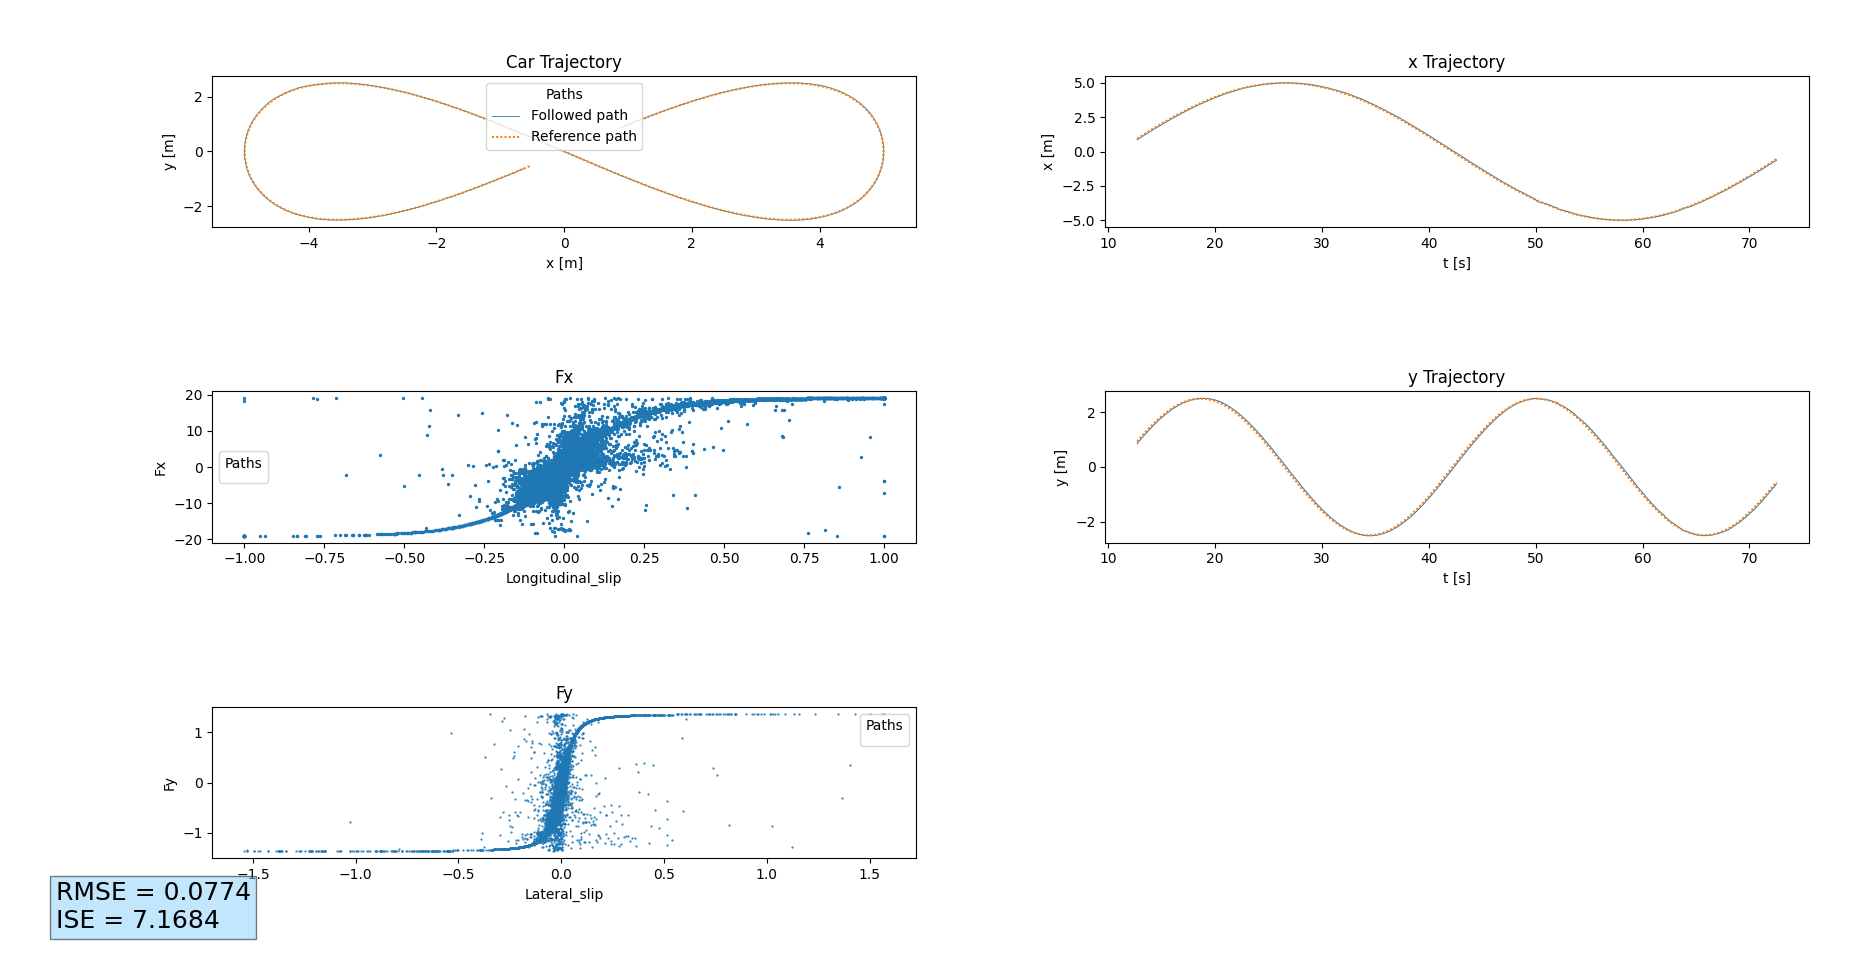
\includegraphics[width=\textwidth]{eight_sim.png}
	\caption{The eight trajectory simulated using Pacejka friction and Gazebo physics models}
\end{figure}

We would also like to present the results obtained by applying the Pacejka modulus correlated with the machine's rectilinear trajectory. \\
As can be seen from the force graph, the values are scattered and not as precise as in the case of the eight trajectory. The reason is related to the parameters used in the calculation of the Pacejka formula. The values chosen were experimentally tested on the eight trajectory, as specified in the section on the plugin.
\begin{figure}[H]
	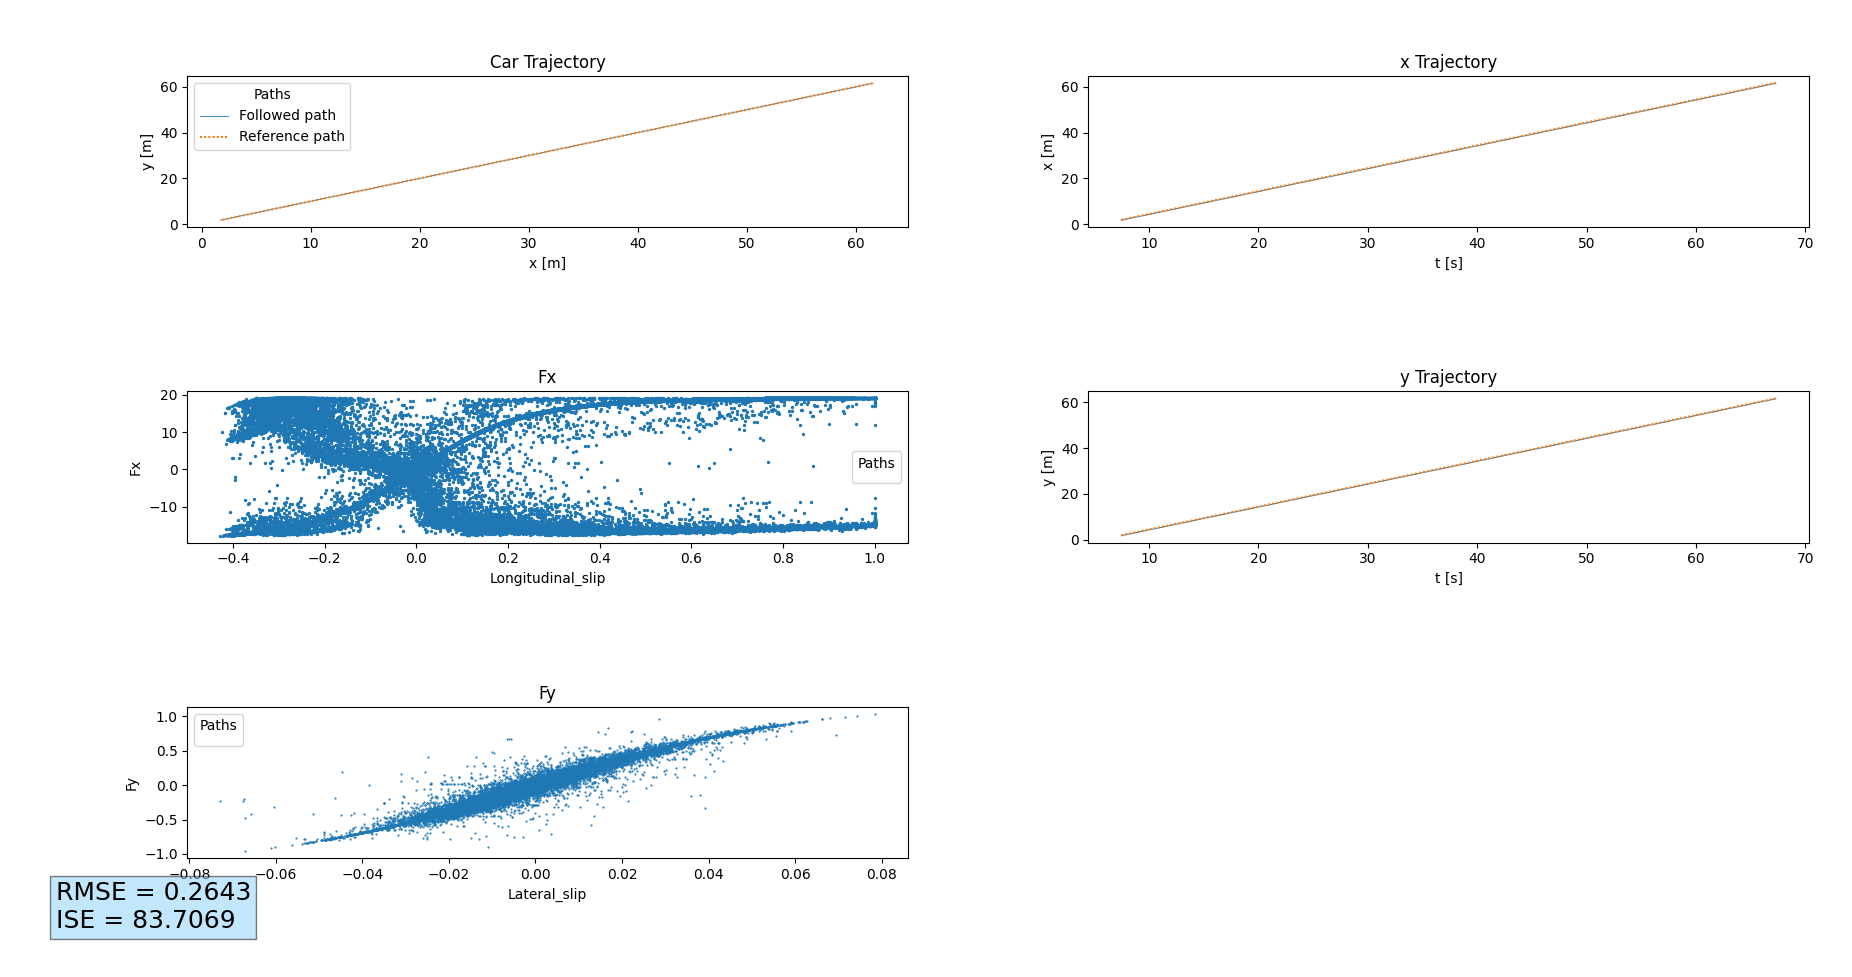
\includegraphics[width=\textwidth]{rect_sim.png}
	\caption{The rectilinear trajectory simulated using Pacejka friction and Gazebo physics models}
\end{figure}

\appendix

\chapter{launch package inclusion}
	
	\usetikzlibrary{arrows.meta}
\begin{figure}[H]
	\makebox[\textwidth][c] 
	{
	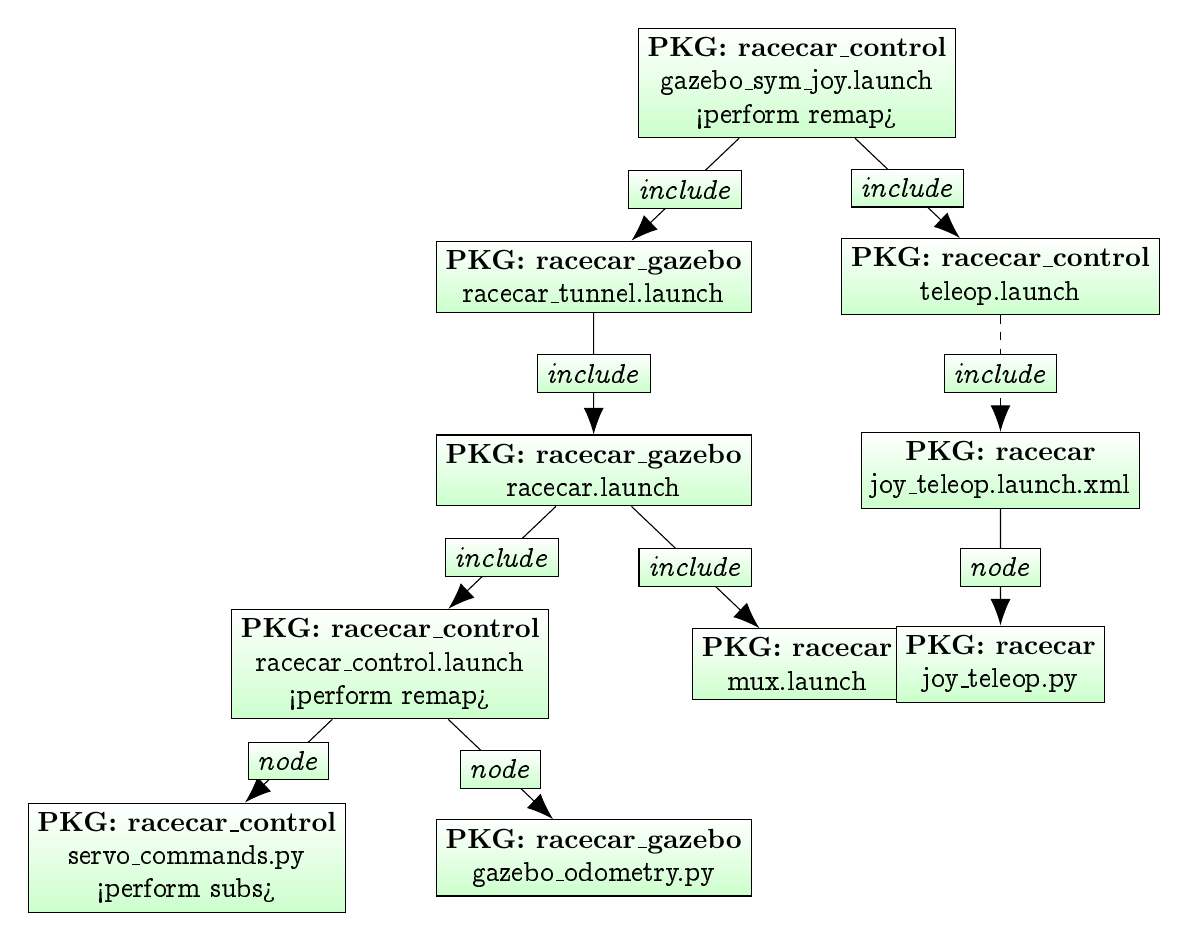
\begin{tikzpicture}[
		scale=0.7,
		level/.style={level distance=10em, sibling distance=21em},
		every node/.style = {
			shape=rectangle, 
			solid,
			draw, 
			align=center,
			top color=white, 
			bottom color=green!20
		},
		norm/.style={edge from parent/.style={-{Latex[scale=2]}, solid, draw}},
		emph/.style={edge from parent/.style={-{Latex[scale=2]}, dashed, draw}}
		]
		\node {\textbf{PKG: racecar\_control} \\ gazebo\_sym\_joy.launch \\ <perform remap>}
		child [norm] { node {\textbf{PKG: racecar\_gazebo} \\ racecar\_tunnel.launch} 
			child [norm] { node {\textbf{PKG: racecar\_gazebo} \\ racecar.launch} 
				child [norm] { node {\textbf{PKG: racecar\_control} \\ racecar\_control.launch \\ <perform remap>} 
					child [norm] { node {\textbf{PKG: racecar\_control} \\ servo\_commands.py \\ <perform subs>} edge from parent node {\textit{node}} }
					child [norm] { node {\textbf{PKG: racecar\_gazebo} \\ gazebo\_odometry.py} edge from parent node {\textit{node}} }
					edge from parent node {\textit{include}}
				}
				child [norm] { node {\textbf{PKG: racecar} \\ mux.launch} edge from parent node {\textit{include}} }
				edge from parent node {\textit{include}}
			} 
			edge from parent node {\textit{include}}
		}
		child [norm] { node {\textbf{PKG: racecar\_control} \\ teleop.launch} 
			child [emph] { node {\textbf{PKG: racecar} \\ joy\_teleop.launch.xml} 
				child [norm] { node {\textbf{PKG: racecar} \\ joy\_teleop.py} edge from parent node {\textit{node}} }
				edge from parent node {\textit{include}}
			}
			edge from parent node {\textit{include}}
		};
	\end{tikzpicture}
	}
\end{figure}
	
%	\begin{tikzpicture}[
%		sibling distance=18em,
%		every node/.style = {
%			shape=rectangle, 
%			draw, 
%			align=center,
%			top color=white, 
%			bottom color=green!20
%		},
%		edge from parent/.style= {
%			draw,
%			-latex
%		}
%		]
%		\node {\textbf{PKG: racecar\_control} \\ keyboard\_teleop.py \\ <perform publish>};
%	\end{tikzpicture}

\begin{center}
	\begin{tabularx}{\linewidth}{|X|X|X|}
		\hline
		\textbf{Package} & \textbf{File} & \textbf{Remap} \\
		\hline
		racecar & joy\_teleop.launch.xml & (none) \\
		\hline
		racecar & joy\_teleop.py & (none) \\
		\hline
		racecar & mux.launch & (none) \\
		\hline
		racecar\_control & gazebo\_sim\_joy.launch & \parbox[t]{5cm}{\raggedright \textcolor{Green}{REMAP \\ /ackermann\_cmd\_ \\ mux/input/teleop \\ TO \\ /racecar/ackermann\_ \\ cmd\_mux/input/teleop}} \\
		\hline
		racecar\_control & teleop.launch & (none) \\
		\hline
		racecar\_control & racecar\_control.launch & \parbox[t]{5cm}{\raggedright \textcolor{Green}{REMAP \\ /racecar/ack/output \\ TO \\ /vesc/low\_level/ \\ ack/output}} \\
		\hline
		racecar\_control & servo\_commands.py & \parbox[t]{5cm}{\raggedright \textcolor{Green}{SUBSCRIBE \\ /racecar/ackermann\_ \\ cmd\_mux/output}} \\
		\hline
		racecar\_control & keybpard\_teleop.py & \parbox[t]{5cm}{\raggedright \textcolor{Green}{PUBLISH \\ /vesc/achermann\_ \\ cmd\_mux/input/teleop}} \\
		\hline
		racecar\_gazebo & racecar\_tunnel.launch & (none) \\
		\hline
		racecar\_gazebo & racecar.launch & (none) \\
		\hline
		racecar\_gazebo & gazebo\_odometry.py & (none) \\
		\hline
	\end{tabularx}
\end{center}

\end{document}